\documentclass[
		pdftex,
		a4paper,	% page format A4
		12pt,		% font size 12pt 
		DIV=calc,
		oneside,	% enable one side
		BCOR5mm,	% add additional padding
		english,	% set language to english
		toc=bibliography,	% include bibliography in TOC
		halfparskip,
		chapterprefix,
		numbers=noenddot,
		titlepage
	]
	{scrbook}   
% ----- weitere Optionen 
%draft,			% Entwurfsmodus zum Anzeigen zu leerer/voller Boxen 
%DIV=calc
%DIV12,			% Seitengröße (siehe Koma Skript Dokumentation !) 
%BCOR5mm,		% Zusätzlicher Rand auf der Innenseite 
%twoside,		% Seitenränder werden an doppelseitig angepasst 
%fleqn,			% Formeln werden linksbündig (und nicht zentriert) angezeigt 
%titlepage,		% Titel wird in einer 'titlepage' Umgebung gesetzt 
%bigheadings,	% Große Überschriften (normal, small-headings) 
%halfparskip-	% Absatz wird nicht eingerückt, dafür aber um eine halbe Zeile nach unten gerückt
%
%---------------------------------------------------
%----- Packages
%---------------------------------------------------
%

\usepackage{layouts}
\usepackage{xcolor,colortbl}
\usepackage{arydshln}
\definecolor{usethiscolorhere}{rgb}{0.92,0.92,0.92}
\usepackage[
		style=numeric,
		citestyle=numeric,
		maxalphanames=1,
		maxcitenames=2,
		backend=bibtex,
		doi=false,
		isbn=false,
		url=false
	]
	{biblatex}
\usepackage[
		font=small,
		format=plain,
		labelfont=bf,
		up,
		textfont=small,
		justification=justified,
		singlelinecheck=false
	]
	{caption}
\usepackage{subcaption}
\usepackage{standalone}
\usepackage{lscape}
\usepackage[T1]{fontenc} 
\usepackage[utf8]{inputenc}
\usepackage[english]{babel} 
\usepackage{ae} 
\usepackage{epigraph}
\usepackage{acronym}
\usepackage[toc,page]{appendix}
\usepackage{fancyhdr} % Define simple headings 
\usepackage{xcolor}
\usepackage{url}
\usepackage{listings}
\usepackage{vmargin} % Adjust margins in a simple way
\usepackage{color}
\usepackage{colortbl}
\usepackage{amsmath}
\usepackage{amssymb}
\usepackage{csquotes}
\usepackage{wrapfig} % Paket zur Positionierung einbinden
\usepackage[pdftex]{graphicx}
\usepackage{pgfplots}  
\usepackage{smartdiagram}
\usepackage{metalogo}
\usetikzlibrary{mindmap,trees}
%\usepackage{dtklogos}
\usepackage{hyperref} % turn all your internal references into hyperlinks
%\usepackage[pdfstartview=FitH,pdftitle={<<Titel der Arbeit>>}, pdfauthor={<<Autor>>}, pdfkeywords={<<Schlüsselwörter>>}, pdfsubject={<<Titel der Arbeit>>}, colorlinks=true, linkcolor=black, citecolor=black, urlcolor=black, hypertexnames=false, bookmarksnumbered=true, bookmarksopen=true, pdfborder = {0 0 0}]{hyperref}
%
% table settings 
\usepackage{booktabs}  
\usepackage{tabularx}
\usepackage{array}   
\usepackage{float}
\usepackage{rotating}
\usepackage{longtable}
\usepackage{pdflscape}
\usepackage{multirow} %multi row
\usepackage{rotating} %for rotating table
\usepackage{color}

\usepackage{tikz}
\usetikzlibrary{positioning}
\usetikzlibrary{shapes.geometric}
\usetikzlibrary{shapes.misc}

\usepackage{framed} 

%---------------------------------------------------
%----- Bibliography setup
%---------------------------------------------------
%
%\bibliographystyle{ieetr}  % citation style
\bibliography{references} % bib file

% the following is needed for syntax highlighting
  
\definecolor{dkgreen}{rgb}{0,0.6,0}
\definecolor{gray}{rgb}{0.5,0.5,0.5}
\definecolor{mauve}{rgb}{0.58,0,0.82}

\definecolor{git_keyword}{HTML}{000000} 
\definecolor{git_key}{HTML}{108888}
\definecolor{git_string}{HTML}{DD1144}
\definecolor{git_tag}{HTML}{121289}
\definecolor{git_attribute}{HTML}{0A8585}
 
\lstdefinelanguage{JSON}{
	keywords={false,true},
	alsoletter=0123456789.,
  	sensitive=false,
  	morecomment=[l]{//},
  	morecomment=[s]{/*}{*/},
  	morestring=[b]',
  	morestring=[b]",
  	keywordstyle=\color{git_key}\bfseries,
    commentstyle=\color{git_string},
	stringstyle=\color{git_string},
}

\lstdefinelanguage{HTML}{
    sensitive=true,
    keywords=[1]{svg, g, path, image},
    otherkeywords={<, \/>, >},   
    keywords=[2]{class, xmlns, xmlns:xlink, xlink:href, width, height, d, x, y},   
    morecomment=[l]{//},
    morecomment=[s]{/*}{*/},
    morecomment=[s]{<!}{>},
    morestring=[b]',
    morestring=[b]",    
    alsoletter={-},
    alsodigit={:},
    keywordstyle=[1]\color{git_tag}\bfseries,
   	keywordstyle=[2]\color{git_attribute},
    commentstyle=\color{git_string},
	stringstyle=\color{git_string},
}

\lstset{
   	backgroundcolor=\color{white},
   	frame=tb,
   	rulecolor=\color{darkgray},    
   	basicstyle=\footnotesize,
   	extendedchars=true,
   	showstringspaces=false,
   	showspaces=false,
   	showtabs=false,
   	numbers=none,
   	tabsize=2,
   	breaklines=true,
   	captionpos=b
}

%
%---------------------------------------------------
%----- PDF and document setup
%---------------------------------------------------
%
\setlength{\parskip}{6pt}
\hypersetup{
	pdftitle={Temporal Analysis of Honey Bee interaction Networks based on Spatial Proximity },  % please, add the title of your thesis
    pdfauthor={Alexa Schlegel},   % please, add your name
    pdfsubject={Master thesis, Institute of Computer Science, Freie Universität Berlin}, % please, select the type of this document
    pdfstartview={FitH},    % fits the width of the page to the window
    pdfnewwindow=true, 		% links in new window
    colorlinks=false,  		% false: boxed links; true: colored links
    linkcolor=red,          % color of internal links
    citecolor=green,        % color of links to bibliography
    filecolor=magenta,      % color of file links
    urlcolor=cyan           % color of external links
}
%
%---------------------------------------------------
%----- Customize header and footer\pagestyle{fancy} 
%---------------------------------------------------

\fancypagestyle{plain}{ % 'plain' page style (used for first page of chapter)
  \fancyhf{} % clear all header and footer fields
  \fancyfoot[LE,RO]{\thepage}
}

\pagestyle{fancy}

\fancyhf{}  % delete all existing header formating
\fancyhead[LE,RO]{\leftmark}  % represent the current chapter heading in uppercase
\renewcommand{\chaptermark}[1]{ % adapt the shown chapter name: show it in lower case and with chapter number 
\markboth{\thechapter.\ #1}{}}   

%\fancyhead[RO]{\rightmark}   % % represent the current section heading in uppercase 
\renewcommand{\sectionmark}[1]{% adapt the shown section name: show it in lower case and with section number 
\markboth{\thesection.\ #1}{}}

\renewcommand{\headrulewidth}{0pt} % remove lines from header
\renewcommand{\footrulewidth}{0pt} % remove lines from header

\newcommand{\tab}{\hspace*{2em}}

% Source http://tex.stackexchange.com/a/32690
\newcolumntype{R}[2]{%
    >{\adjustbox{angle=#1,lap=\width-(#2)}\bgroup}%
    l%
    <{\egroup}%
}
\newcommand*\rot{\multicolumn{1}{R{45}{1em}}}% no optional argument here, please!

\fancyfoot{} % delete all existing footer formating
\fancyfoot[LE,RO]{\thepage} 

%%%%%%%%%%%%%%%%%%%%%%%%%%%%%%%%%%%%%%%%%%%%%%%%%%%%%%%%%%%%%%%%%%%%%%%%%%%%%%
% ---- Namen der Links im Dokument
%\addto\captionsngerman{\renewcommand{\figurename}{\small{\textbf{Abb.}}}}
%\addto\captionsngerman{\renewcommand{\tablename}{Tab.}}
%\addto\captionsngerman{\captionsetup{figurewithin = section}}
%\addto\captionsngerman{\captionsetup{font=small, labelfont=bf}}

%
%---------------------------------------------------      
%----- Settings for word separation  
%---------------------------------------------------      
% Help for separation (from package babel, section 22)):
% In german package the following hints are additionally available:
% "- = an explicit hyphen sign, allowing hyphenation in the rest of the word
% "| = disable ligature at this position. (e.g., Schaf"|fell)
% "~ = for a compound word mark without a breakpoint (e.g., bergauf und "~ab)
% "= = for a compound word mark with a breakpoint, allowing hyphenation in the composing words
% "" = like "-, but producing no hyphen sign (e.g., und/""oder)
%
% Describe separation hints here:
\hyphenation{
% Pro-to-koll-in-stan-zen
% Ma-na-ge-ment  Netz-werk-ele-men-ten
% Netz-werk Netz-werk-re-ser-vie-rung
% Netz-werk-adap-ter Fein-ju-stier-ung
% Da-ten-strom-spe-zi-fi-ka-tion Pa-ket-rumpf
% Kon-troll-in-stanz
}

\usepackage{ragged2e}  % for '\RaggedRight' macro (allows hyphenation)
\newcolumntype{Y}{>{\RaggedRight\arraybackslash}X}


%%%%%%%%%%%%%%%%%%%%%%%%%%%%%%%%%%%%%%%%%%%%%%%%%%%%%%
% The content part of the document starts here! %%
%%%%%%%%%%%%%%%%%%%%%%%%%%%%%%%%%%%%%%%%%%%%%%%%%%%%%%

\begin{document}
\frontmatter 

%\pagenumbering{alph} % even though, these page numbers are not visible there are necessary to have unique page numbers 
% ---------------------------------------------------
% ----- Title page of the template
% ----- for Bachelor-, Master thesis and class papers
% ---------------------------------------------------
%  Created by C. Müller-Birn on 2012-08-17, CC-BY-SA 3.0.
%  Freie Universität Berlin, Institute of Computer Science, Human Centered Computing. 
%
\begin{titlepage}

\title{
{\small Master Thesis, Institute of Computer Science, Freie Universität Berlin}\\
{\small Biorobotics Lab, Intelligent Systems and Robotics}\\
[6ex]
{\LARGE Temporal Analysis of\\ Honey Bee Interaction Networks\\Based on Spatial Proximity\\}
\vspace{2ex}
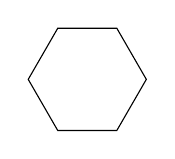
\begin{tikzpicture}[node distance=1cm]
  \node[regular polygon, regular polygon sides=6, shape aspect=0.5, minimum width=1.5cm, minimum height=1cm, draw] (reg) {};
\end{tikzpicture}\\
}

\author{
{\emph{\normalsize Alexa Schlegel}}\\
{\normalsize Matriculation number: 4292909}\\
{\normalsize alexa.schlegel@fu-berlin.de}\\ 
[15ex]   
{\normalsize Supervisor: Prof. Dr. Tim Landgraf, Freie Universität Berlin}\\
{\normalsize Second Supervisor: Dr. Philipp Hövel, Technische Universität Berlin}\\
}
\vspace{6ex}
\date{\normalsize Berlin, \today}
 
\maketitle  


\end{titlepage}
% ---------------------------------------------------
% ----- Declaration of the template
% ----- for Bachelor-, Master thesis and class papers
% ---------------------------------------------------
%  Created by C. Müller-Birn on 2012-08-17, CC-BY-SA 3.0.
%  Freie Universität Berlin, Institute of Computer Science, Human Centered Computing. 
%
\pagestyle{empty}

\subsection*{Eidesstattliche Erklärung}

Ich versichere hiermit an Eides Statt, dass diese Arbeit von niemand anderem als meiner Person verfasst worden ist. Alle verwendeten Hilfsmittel wie Berichte, Bücher, Internetseiten oder ähnliches sind im Literaturverzeichnis angegeben, Zitate aus fremden Arbeiten sind als solche kenntlich gemacht. Die Arbeit wurde bisher in gleicher oder ähnlicher Form keiner anderen Prüfungskommission vorgelegt und auch nicht veröffentlicht.
\par\bigskip  
\noindent Berlin, den \today

\vspace{1.2cm}

\noindent Alexa Schlegel

\cleardoublepage
%%*******************************************************
% Dedication
%*******************************************************
\thispagestyle{empty}
%\phantomsection 

\pdfbookmark[1]{Dedication}{Dedication}

\vspace*{3cm}

\begin{center}
    Everything we hear is an opinion, not a fact. \\ Everything we see is a perspective, not the truth.  \\ \medskip
    --- Marcus Aurelius 
\end{center}

\medskip

\begin{center}
    Dedicated to my parents and my brother.
\end{center}

%---------------------------------------------------
%----- Abstracts in English and German   
%---------------------------------------------------

% ---------------------------------------------------
% ----- Abstract (English)
% ---------------------------------------------------
%  Freie Universität Berlin, Institute of Computer Science, Human Centered Computing. 
%
\pagestyle{empty}
\providecommand{\keywords}[1]{\textbf{\textit{Keywords---}} #1}

\subsection*{Abstract}
The BeesBook system automatically tracks individual honey bees inside a hive over their entire life and provides a high-resolution dataset of bee movements of a single colony.
This thesis focuses on the inference of interaction networks, by implementing a network pipeline.
Spatial proximity is using as an indicator for interactions between bees.
Social network analysis methods were applied to investigate the static and dynamic properties of the resulting social networks of honey bees on a global, intermediate and local level.
The resulting networks were characterized by a low hierarchical structure and a high density.
The global structure of the colony seems to be stable over time.
The local structure is highly dynamic, as bees change communities as they age.
Communities in the honey bee network represent age groups with a high spatial fidelity.
The findings are in line with established state of research that a colonies organization is shaped by the age-based task division of individuals.
The results of the analysis validate the implemented pipeline and inferred networks and consequently provide an excellent foundation for future work focusing more on temporal network analysis aspects.

\keywords{social insects, spatial proximity network, social network, interaction network, honey bee, behavioural tracking, Apis mellifera, community detection, social network analysis}

\cleardoublepage
 
                                          
%---------------------------------------------------
%----- Table of content   
%---------------------------------------------------
\tableofcontents
%\setcounter{tocdepth}{3}   % reduce the included sections in the table of content

%---------------------------------------------------
%----- Main part
%---------------------------------------------------
\mainmatter

\pagestyle{fancy} 

%%%%%%%%%%%%%%%%%%%%%%%%%%%%%%%%%%%%%%%%%%%%%%%%%%%%%%%%%%%%%%%%%%%%%%%%%%%%%%%
%%%%%%%%%%%%%%%%%%%%%%%%%%%%%%%%%%%%%%%%%%%%%%%%%%%%%%%%%%%%%%%%%%%%%%%%%%%%%%%
%%%%%%%%%%%%%%%%%%%%%%%%%%%%%%%%%%%%%%%%%%%%%%%%%%%%%%%%%%%%%%%%%%%%%%%%%%%%%%%
%%%%%%%%%%%%%%%%%%%%%%%%%%%%%%%%%%%%%%%%%%%%%%%%%%%%%%%%%%%%%%%%%%%%%%%%%%%%%%%
\chapter{Introduction}
\label{ch:intro}
%%%%%%%%%%%%%%%%%%%%%%%%%%%%%%%%%%%%%%%%%%%%%%%%%%%%%%%%%%%%%%%%%%%%%%%%%%%%%%%
%%%%%%%%%%%%%%%%%%%%%%%%%%%%%%%%%%%%%%%%%%%%%%%%%%%%%%%%%%%%%%%%%%%%%%%%%%%%%%%
%%%%%%%%%%%%%%%%%%%%%%%%%%%%%%%%%%%%%%%%%%%%%%%%%%%%%%%%%%%%%%%%%%%%%%%%%%%%%%%
%%%%%%%%%%%%%%%%%%%%%%%%%%%%%%%%%%%%%%%%%%%%%%%%%%%%%%%%%%%%%%%%%%%%%%%%%%%%%%%

A social insect society is formed by thousands of individuals, which continuously move and interact with each other inside a dark nest. 
Honey bees are organized in colonies, which form a complex and dynamical system.
Observing individual honey bees and their interactions with each other is, therefore, vital for understanding collective behavior and the organization of tasks within the colony.

Within the BeesBook project of the Biorobotics Lab of Freie Universität Berlin~\textcite{wario2015automatic} developed technologies to automatically track all individuals of a honey bee (Apis mellifera) colony, that are inside the honeycomb.

Shortly after hatching, each bee is marked on their thorax by using circular 12-bit tags (figure~\ref{fig:markers}) and then added to the observation colony. Four cameras observe the comb over a period of nine weeks, by capturing approximately three frames per second. An image analysis pipeline evaluates each frame automatically. The resulting data set contains, for each frame, the exact position of each detected bee on the honeycomb, and its age.

In this thesis, worker-worker interaction networks, based on spatial proximity, are derived from the described data set. Each node in the network is a bee, and a link between two nodes results if two bees are located close to each other over a specified period.
The networks are time-aggregated, which means one network represents the data of multiple frames.

After extracting the temporal networks, social network analysis methods are applied to determine the characteristics of the resulting networks and its communities.

\begin{figure}[htb]
	\centering
	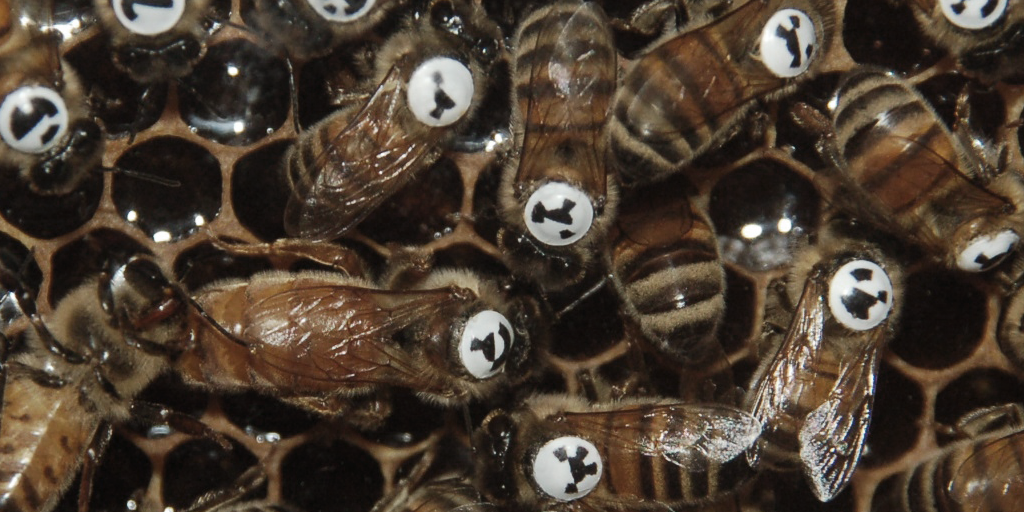
\includegraphics[width=1.0\textwidth]{Figures/markers}
	\caption{Tagged bees inside the observation hive.}
	\label{fig:markers}
\end{figure}

%%%%%%%%%%%%%%%%%%%%%%%%%%%%%%%%%%%%%%%%%%%%%%%%%%%%%%%%%%%%%%%%%%%%%%%%%%%%%%%
%%%%%%%%%%%%%%%%%%%%%%%%%%%%%%%%%%%%%%%%%%%%%%%%%%%%%%%%%%%%%%%%%%%%%%%%%%%%%%%
\section{Motivation}
%%%%%%%%%%%%%%%%%%%%%%%%%%%%%%%%%%%%%%%%%%%%%%%%%%%%%%%%%%%%%%%%%%%%%%%%%%%%%%%
%%%%%%%%%%%%%%%%%%%%%%%%%%%%%%%%%%%%%%%%%%%%%%%%%%%%%%%%%%%%%%%%%%%%%%%%%%%%%%%

Colonies of social insects consist of a vast number of individuals. Due to technical and observational limitations, most studies in the field of animal social network analysis, related to insects, analyze only a small subset of a colonies' life.
Usually, the reduction is carried out on three levels (1) time and resolution, (2) space, and (3) number of individuals.


[TODO: umarbeiten!!!, einzelne Studien müssen in related work, (A) method/approach: network analysis, network properties and communities; (B) animals: focus bees, but also considering social insects studies; (C) tracking methods: manual tracking and automatic tracking; automatic tracking, more inclusive, temporal development, dadurch Mehrwert, d.h. gap of knowledge im Bereich: Social Network Analysis von Honey Bees with automatic tracking and long term development, hm... Studies in den anderen Bereichen (automatic tracking and social insects, manual tracking bees, manual tracking of social insects, with network science approach already exists). Automatic tracking allows shifting more towards the temporal and dynamic investigation.]

Labeling only a subset of the colonies individuals, a short observation period, low res\-olution and manually extracting information from photos or videos is very common in behavioral sciences~\cite{naug2008structure, quevillon2015social}.

\textcite{baracchi2014socio} observed 300 bees out of a colony with 4000 individuals over a period of ten hours. One of the two sides of the hive was observed by taking a photo each minute. Coloured numbered discs were used for individually marking bees. The analysis of a weighted and undirected worker-worker interaction network revealed a highly compartmentalized structure inside the honey bee colony. Depending on the age, bees occupy different areas of the comb and correspond to different tasks. Also, the contact is limited within groups. \textcite{blonder2011time} color painted all individuals of ant colonies (size 6-90 for each colony) and filmed the colonies for 30 minutes. Interactions between individuals were manually extracted by watching the videos. Using time-ordered (dynamic) networks they analyzed the temporal and spatial dynamics of information flow.

Recently, automated tracking of insects has become technically feasible~\cite{wario2015automatic, crall2015beetag, fiala2005comparing}.
Using automated high resolution tracking data, which includes all individuals of the complete comb over a long time period allows for more advanced analysis focusing on temporal dynamics.
\textcite{mersch2013tracking} automatically tracked all individuals of six ant colonies over a period of 41 days. Applying the Infomap community detection algorithm to the physical contact networks for each day, revealed three distinct and robust groups. Each group represents a functional behavioral unit, with individuals changing groups as they age.

The majority of social insect interaction networks studies, due to previously technical limitations, aggregate temporal tracking data into a single static network~\cite[Chapter~15]{krause2014animal}.
Automatic tracking allows shifting more towards the temporal and dynamic investigation.


\section{Research Goal}
The aim of this thesis is to investigate whether the provided data set of tracked honey bees is useful for creating worker-worker interaction networks using spatial proximity as an indicator for interactions between bees. Thus, I need to implement a pipeline to extract networks out of the given data set. Furthermore, I want to find out if the resulting networks are suitable for social network analysis.

I want to achieve my research goals by answering the following questions:

\begin{enumerate}
\item \emph{Is it possible to infer (temporal) networks with the provided honey bee tracking data?}\\
What challenges and limitations does the data set imply?
What pipeline parameters are necessary?
\item \emph{What kind of worker-worker interaction networks emerge and how are they structured?}\\
What is their topology?
What properties are characteristic and how do they differ from randomly generated networks?
\item \emph{Does the network display a meaningful community structure?}\\
How are the identified communities characterized?
Do they reflect already known colony behavior concerning age and spatial distribution?
\item \emph{How do these communities develop over time?}\\
Are they stable regarding their properties?
How do members move between communities?
\end{enumerate}

This work is meant to be the foundation to answer further more specific biological research questions using a network science approach to study and evaluate the complex system of honey bee colonies and their collective behavior.

\section{Methodology}
The methodology of this thesis follows a standard explorative data analysis procedure, mainly to understand the given data set and estimate its quality. The elaborated characteristics of the dataset are then used to define parameters and the procedure of network extraction. This pipeline is developed, tested and then refined in an iterative process. Test results lead to new or changing functional requirements of the pipeline.

The resulting networks are evaluated using the following approaches:

\begin{itemize}
\item Investigation of pipeline parameters' effects,
\item Quality inspection by examining the age of bees,
\item Comparison with a random graph model,
\item Repeatability of known results and facts concerning community structures.
\end{itemize}

\section{Outline}
This thesis is organized as follows. Chapter~\ref{ch:bg} gives a short introduction into social network analysis (SNA) and defines network measures, terms, and algorithms used throughout this work.
In chapter~\ref{ch:relatedwork}, a brief summary of the current state of research concerning social insect networks, temporal networks and community detection in animal social networks is given.
Chapter~\ref{ch:approach} describes my research approach in general and how the pipeline infers networks out of the given dataset, what steps are needed and what parameters it uses.
Also, I explain and justify what decisions I took during the network analyses and community detection process.
Chapter~\ref{ch:results} reports the results of the network analysis and the characteristics of the extracted communities.
Finally, in chapter~\ref{ch:conclusion} I explore the results, discuss limitations and conclude with directions for future work.
\chapter{Theretical Background}
The following chapter gives a short introduction into social network analysis (SNA). It introduces animal interaction networks as a special type of network. It defines terms and concepts used throughout this work and explains networks metrics and algorithms of which we will make use of.

Social network analysis is a way of mapping and measuring specific relationships and flows between entities

mapping and measuring of relationships and flows between people, groups, organizations, computers, URLs, and other connected information/knowledge entities. 
\\
Social network analysis (SNA) is the process of investigating social structures through the use of network and graph theories.[1] It characterizes networked structures in terms of nodes (individual actors, people, or things within the network) and the ties, edges, or links (relationships or interactions) that connect them. 
 
number of nodes/vertices $N$ (size of the network)\\
number of links/edges $L$\\
$D$ is density $D=\frac{2L}{N(N-1)}$
$k$ degree of a node $n$, $k_i$ of $n_i$\\
$ \langle k  \rangle$ average degree\\
definitions taken from~\textcite{barabasi2016network}\\

$\langle C \rangle$ average clustering coefficient\\

* number of nodes $N$\\
* number of links $L$\\
* density $D$\\
* average degree $ \langle k  \rangle$\\
* average weighted degree, average strength $\langle s \rangle$\\ 
* max and min (weighted) degree\\
* global clustering coefficient $C_\Delta = \frac{3 \times \texttt{number of triangles}}{\texttt{number of connected triples}}$ (transiticvity undirected)~\cite{wasserman1994social}\\

* Number of components (Connesctedness): components = subnetworks, A component is a subnet of nodes in a network, so that there is a path between any two nodesthat belong to teh component, but one cannot addany more nodes to it that would have the same property.\\

* Average shortest path (average path length) $\langle d \rangle$: The average of the shortest path between all pairs of nodes.\\

* Diameter $d_{\texttt{max}}$:The longest shortest path , or the distance between the two furthest nodes.\\




\section{Animal Interaction Networks}

Networks where individuals are nodes and edges are defined as interaction events between individuals are called \emph{interaction networks}, sometimes also contact networks. 
Those interactions used as an edge can be of different types~\cite{charbonneau2013social}:

\begin{itemize}
\item spatial proximity~\cite{jeanson2012long, otterstatter2007contact},
\item physical contact (usually with antennae, “antennation”)~\cite{mersch2013tracking} [TODO anschauen: 10, 67, 80]
\item a food exchange event (trophallaxis) [TODO anschauen: 15, 68, 69, 93]
\item or specific communication signals [TODO anschauen: 38, 56]
\end{itemize}

directed and undirected\\
weighted and unweighted\\

define proximity/association\\

\subsection{Terminology}
Basic terms\\

Graph: a set of nodes and a set of relationships between the
nodes, given by a matrix or visualized as a picture showing
dots connected by lines\\

Node: a component of a network with known relationships
to others in the graph model representing the network; in
a social network, this can be an individual (person or animal)
or group; also called a vertex or point\\

Path length: the shortest number of ties between two nodes\\

Sociomatrix: for a group with n members, an nn matrix
with each group member along the vertical and horizontal
axes and each entry in the grid as the weight of the social relationship,
if any, between the two intersecting individuals\\

Tie: a relationship between two components of a network,
where the two related components are nodes in the graph
model representing the network; in a social network, these
can be any sort of social relationship, such as social interactions
or information transfer; also called an edge or link\\

Individual (local) measures\\

Betweenness centrality: centrality based on the number of
shortest paths between every pair of other group members
on which the focal individual lies\\

Centrality: a measure of an individual’s structural importance
in a group based on its network position\\

Closeness centrality: centrality based on the shortest path
length between a focal individual and all other members of
the social group\\

Degree centrality: centrality based on the number of direct
ties an individual has\\

Indegree (reception): the number of ties directed towards
an animal, e.g. the number of social interactions it receives\\

Node degree: the number of ties a focal animal has; the
number of other animals with which the focal individual
interacts\\

Outdegree (emission): the number of ties originating from
an animal, e.g. the number of social interactions it initiates\\

Intermediate measures\\

Clustering coefficient: the density of the subnetwork of a focal
individual’s neighbours; the number of ties between
neighbours is divided by the maximal possible number of
ties between them\\

Cliquishness: how much the network is divided into cohesive
subgroups; a clique is a set of nodes where each node
is directly tied to each other\\

Group measures\\

Average path length: the average of all path lengths between
all pairs of nodes in the network\\

Density: the number of realized ties divided by the number
of possible ties in the network\\

Diameter: the longest path length in the network\\
\textcite{wey2008social}

\section{Network Metrics and Algorithms}
Degree Distribution\\
Degree Centrality, Closeness Centrality, Betweenness Centrality\\
Clustering Coefficient\\
Modularity\\

Proximity (distance), strength, disparity, closeness, and betweennes are taken from \textcite{jeanson2012long}.\\

\paragraph*{Measures for weighted networks}
strength $S_i$ measures the total weight of edges connected to a node $i$ and is definded as $S_i = \sum_{j=1}^{n}w_ij$ according to~\textcite{barrat2004architecture}\\
closeness, computed using Dijkstra’s algorithm with that edge attribute as the edge weight~\cite{newman2001scientific}\\
betweenness using dijkstra~\cite{brandes2001faster}\\

weighted clustering coefficient and weighted average clustering coefficient~\cite{saramaki2007generalizations}\\

\paragraph*{Disparity}
\url{https://github.com/aekpalakorn/python-backbone-network}
Low values of disparity indicated that the weights of associations were of the same order and, consequently, that ants interacted homogeneously with all nestmates. In contrast, privileged associations between ants were evidenced by relatively large values of disparity showing the dominance of a few weights over the others.~\cite{barthelemy2005characterization}

Disparity: For a given node i   with connectivity  ki  and strength  si  different situations can arise. All weights  wij  can be of the same order  si/ki . In contrast, the most heterogeneous situation is obtained when one weight dominates over all the others. A simple way to measure this “disparity” is given by the quantity  Y2  introduced in other context [12] ;  [13];

$$Y_2(i)=\sum_{j\in \Theta(i)} (\frac{w_ij}{s_i})^2$$

\paragraph*{Centrality measures}
betweenness and closeness

\paragraph{Network Reduction algorithms (backboning)}
k-core decomposition\\
minimum spanning tree\\
Global weight treshold\\
Disparity Filter\\


\section{Temporal Networks}

\section{Community Detection}

[TODO: Definition Community, densly connected supgraph (strong, weak, communities, mit welcher Definition arbeite ich)]



~\cite{newman2006finding}\\

\section{Communities in evolving networks}
\label{sec:bg:tracking}
According to \textcite{aynaud2013communities} and \textcite{brodka2014community} there are three main approaches for community detection in temporal networks (also called community tracking): (1) using a static community detection algorithm on several snapshots and then solving a matchig problem, (2) using algorithms who are directly suited for temporal networks and (3) using incremental or online algorithms when processing data streams. For each of the three approaches, several mehods already exist.

As community tracking is not the main focus of this work, I chose to apply the most intuitive approach aout of approach (1): detecting static communities for each snapshot and then matching those communities using set theory.  Two communities at successive timesteps are matched if they share enough nodes. The \emph{match value} (between 1 and 0) between two communities $C$ and $D$ according to~\cite{hopcroft2004tracking} is defined as:

\begin{equation}
\label{eq:match}
\texttt{match}(C,D) = \texttt{min}\left( \frac{\textbar C\cap D \textbar}{\textbar C\textbar }, \frac{\textbar C\cap D \textbar}{\textbar D \textbar }\right)
\end{equation}

A high match value accurse, when two communities share a lot of nodes and are of a similar size. Communities with the highest value are matched. A threshold should be applied to more precicley define what ``share enough nodes'' means.

%%%%%%%%%%%%%%%%%%%%%%%%%%%%%%%%%%%%%%%%%%%%%%%%%%%%%%%%%%%%%%%%%%%%%%%%%%%%%%%
%%%%%%%%%%%%%%%%%%%%%%%%%%%%%%%%%%%%%%%%%%%%%%%%%%%%%%%%%%%%%%%%%%%%%%%%%%%%%%%
\section{Related Studies}
\label{ch:relatedwork}
%%%%%%%%%%%%%%%%%%%%%%%%%%%%%%%%%%%%%%%%%%%%%%%%%%%%%%%%%%%%%%%%%%%%%%%%%%%%%%%
%%%%%%%%%%%%%%%%%%%%%%%%%%%%%%%%%%%%%%%%%%%%%%%%%%%%%%%%%%%%%%%%%%%%%%%%%%%%%%%

Studies using a network analysis approach focusing on interaction networks\footnote{Studies using worker-task, worker-nestarea, nestarea-nestarea or other bipartite networks are excluded.} to investigate the behavior of social insects, especially honey bees are relevant for my work.
I mainly reviewed studies mentioned in the survey papers of \textcite{Pinter-Wollman2014}, \textcite[chapter~15]{krause2014animal} and \textcite{charbonneau2013social}.

The most relevant studies were classified by:

\begin{itemize}
\item \textbf{Type of analysis}\\
temporal or static analysis using automated or manual tracking over a long or short term
\item \textbf{Studied species}\\
honey bees or other social insects
\end{itemize}

I reviewed the limitations of the studies in regards to time, space, and the number of tracked individuals. Table~\ref{tab:studies} (Appendix~\ref{ch:appendix}) summarizes the selected studies and the characteristics of: duration of study, observation period, sampling resolution, the number of colonies, the number of marked individuals, and space limitations.
I also recorded whether the studies included age cohorts in their analysis and listed the software tools used for network analysis.

Within the scope of my literature review, I found a lot of studies in the field of static network analysis of ants~\cite{greenwald2015ant,pinter2011effect,quevillon2015social,formica2012fitness,waters2012information,sendova2010emergency}, wasps~\cite{naug2009structure} and bumblebees~\cite{otterstatter2007contact}, but only a few related to honey bees~\cite{baracchi2014socio,naug2008structure,scholl2011olfactory,naug2007experimentally}.
I did not find any studies focused on temporal aspects of honey bee colonies, but I did find several studies focused on temporal aspects of ant colonies~\cite{mersch2013tracking,blonder2011time,jeanson2012long}.

%%%%%%%%%%%%%%%%%%%%%%%%%%%%%%%%%%%%%%%%%%%%%%%%%%%%%%%%%%%%%%%%%%%%%%%%%%%%%%%
%%%%%%%%%%%%%%%%%%%%%%%%%%%%%%%%%%%%%%%%%%%%%%%%%%%%%%%%%%%%%%%%%%%%%%%%%%%%%%%
\subsection{Static Network Analysis of Honey Bee Colonies}
%%%%%%%%%%%%%%%%%%%%%%%%%%%%%%%%%%%%%%%%%%%%%%%%%%%%%%%%%%%%%%%%%%%%%%%%%%%%%%%
%%%%%%%%%%%%%%%%%%%%%%%%%%%%%%%%%%%%%%%%%%%%%%%%%%%%%%%%%%%%%%%%%%%%%%%%%%%%%%%

The most advanced work studying honey bees using a network science approach is by \textcite{baracchi2014socio}.
Their study revealed a highly compartmentalized structure inside the honey bee colony:
Bees organize by age groups, which occupy separate areas of the comb and perform different tasks.
There is limited contact between these groups.

Generally, the theory that bees change tasks over the course of their lifetime, starting as nurses in the nest and ending as foragers outside, termed as temporal polyethism,  is widely accepted and has been studied for a long time~\cite{seeley1982adaptive, johnson2008within, lindauer1952beitrag}.
\textcite{johnson2008within} observed two groups of within-nest bees: young bees responsible for the brood care and middle-aged bees specialized on nectar processing and nest maintenance.
\textcite{seeley1982adaptive} observes four age subcastes among worker bees besides the queen cast: cell cleaning, brood nest, food storage, forager.\\
\textcite{lindauer1952beitrag} defined certain tasks a bee can perform at any given age. Also, a bee can perform several different tasks per day. The bee is flexible and responds to the given needs of the hive. Young bees mostly clean cells and old bees mainly forage, instead middle-aged bees perform several tasks.~\cite{lindauer1952beitrag}

\textcite{baracchi2014socio} use the frequency of interactions between bees as link weights in an undirected worker-worker interaction network.
The body length of a bee defines the radius of spatial proximity.
Baracchi and Cini use the node level measures strength (weighted degree), closeness and eigenvector centrality to investigate the networks.
They also perform a cluster analysis using as similarity the local network measures.
The main shortcomings of their work are sample size and observation frequency. They studied one colony with 4000 individuals, marking only 211 bees from three predefined age cohorts, and observed only one side of the observation hive for ten hours by capturing with a low resolution of one frame per minute.

%%%%%%%%%%%%%%%%%%%%%%%%%%%%%%%%%%%%%%%%%%%%%%%%%%%%%%%%%%%%%%%%%%%%%%%%%%%%%%%

\textcite{scholl2011olfactory} investigated the mechanism behind the emergence of organizational immunity of honey bee colonies by using unweighted, undirected physical contact and trophallaxis networks.
They observed one hour per day, with three days of observation spread over three weeks.
In the field of network analysis, they investigated the interactions between three predefined age cohorts.

%%%%%%%%%%%%%%%%%%%%%%%%%%%%%%%%%%%%%%%%%%%%%%%%%%%%%%%%%%%%%%%%%%%%%%%%%%%%%%%

\textcite{naug2008structure} inspects the network structure of weighted, directed trophallaxis networks using four age cohorts.
He evaluates the changes in transmission dynamics produced by experimental manipulation.
The data set is limited to one hour of observation and only first- and second-order\footnote{The food transfer from the forager to a worker bee is called first level interaction, the food transfer from that worker bee to other bees is called second-order.} trophallaxis interactions are considered.


%%%%%%%%%%%%%%%%%%%%%%%%%%%%%%%%%%%%%%%%%%%%%%%%%%%%%%%%%%%%%%%%%%%%%%%%%%%%%%%
%%%%%%%%%%%%%%%%%%%%%%%%%%%%%%%%%%%%%%%%%%%%%%%%%%%%%%%%%%%%%%%%%%%%%%%%%%%%%%%
\subsection{Temporal Network Analysis of Insect Colonies}
%%%%%%%%%%%%%%%%%%%%%%%%%%%%%%%%%%%%%%%%%%%%%%%%%%%%%%%%%%%%%%%%%%%%%%%%%%%%%%%
%%%%%%%%%%%%%%%%%%%%%%%%%%%%%%%%%%%%%%%%%%%%%%%%%%%%%%%%%%%%%%%%%%%%%%%%%%%%%%%

\textcite{mersch2013tracking} apply similar methods to my work.
They automatically tracked all individuals of six ant colonies over a period of 41 days using a resolution of two frames per second.
For each observation day, the authors extracted time-aggregated weighted contact networks per colony, using antennation as the physical contact event.
They applied the Infomap community detection algorithm to each daily network and revealed three distinct and robust groups.
Each group represents a functional behavioral unit, with ants changing groups as they age.
Except for community detection, they did not use any other network science methods to investigate the network properties.

%%%%%%%%%%%%%%%%%%%%%%%%%%%%%%%%%%%%%%%%%%%%%%%%%%%%%%%%%%%%%%%%%%%%%%%%%%%%%%%

\textcite{jeanson2012long} also used automatic tracking.
His work is focused on the investigation of the temporal stability of spatial proximity networks in four ant colonies over three weeks.
Here, proximity is defined as $\frac{4}{3}$ of an ant’s body length.
Per week and per colony they generated weighted time-aggregated networks, using the total duration of interaction as the link weights.
They investigated the strength, betweenness and closeness centrality and found that the networks are stable over time, without the queen contributing to the network structure.
Also they state that individuals with long lasting interactions seem to have a reduced tendency to move, while mobile ants interact homogeneously with their nestmates.
The observed colonies ranged in size from 55 to 58 individuals.

%%%%%%%%%%%%%%%%%%%%%%%%%%%%%%%%%%%%%%%%%%%%%%%%%%%%%%%%%%%%%%%%%%%%%%%%%%%%%%%

In these studies, each of the observed ant colonies contained a maximum of 200 individuals. This number is relatively small compared to the size of honey bee colonies used in the static analysis approaches.
\chapter{Approach and Implementation}
\label{ch:approach}
%%%%%%%%%%%%%%%%%%%%%%%%%%%%%%%%%%%%%%%%%%%%%%%%%%%%%%%%%%%%%%%%%%%%%%%%%%%%%%%
%%%%%%%%%%%%%%%%%%%%%%%%%%%%%%%%%%%%%%%%%%%%%%%%%%%%%%%%%%%%%%%%%%%%%%%%%%%%%%%
%%%%%%%%%%%%%%%%%%%%%%%%%%%%%%%%%%%%%%%%%%%%%%%%%%%%%%%%%%%%%%%%%%%%%%%%%%%%%%%
%%%%%%%%%%%%%%%%%%%%%%%%%%%%%%%%%%%%%%%%%%%%%%%%%%%%%%%%%%%%%%%%%%%%%%%%%%%%%%%
[TODO: ref this part in introduction, methods part]

This chapter describes the workflow and implementation I applied to reach my research goals.
The preparation and processing of the data are primarily driven by a combination of exploratory and iterative processes.

I primarily follow  Farine's and Whitehead's~\cite{farine2015constructing} steps and key considerations for social network analysis to non-human animal data.
[TODO: steps kurz zusammenfassen, und unterschiede zu mir erklären]
Figure~\ref{fig:process} visualizes the adapted and resulting process.
[TODO: Schritte im Bild nummerieren und im Text verwenden]

In the first step, the data set was analyzed to form a general understanding of the given dataset, its structure, quality, and characteristics.

The results of this investigation are used to build the network by defining nodes, inferring associations, and deriving the parameters for the network pipeline.

The resulting networks are analyzed by using network science tools and methods.
[hier unbedingt methoden aufzählen]																																																																																																						

[TODO: umfomulieren, Begruendun Auswahl der Attribute, und welche Test habe ich genau gemacht.]
For testing underlying hypothesis the networks are attributed with the bees spatial information and their age.

\begin{figure}[htb]
	\centering
	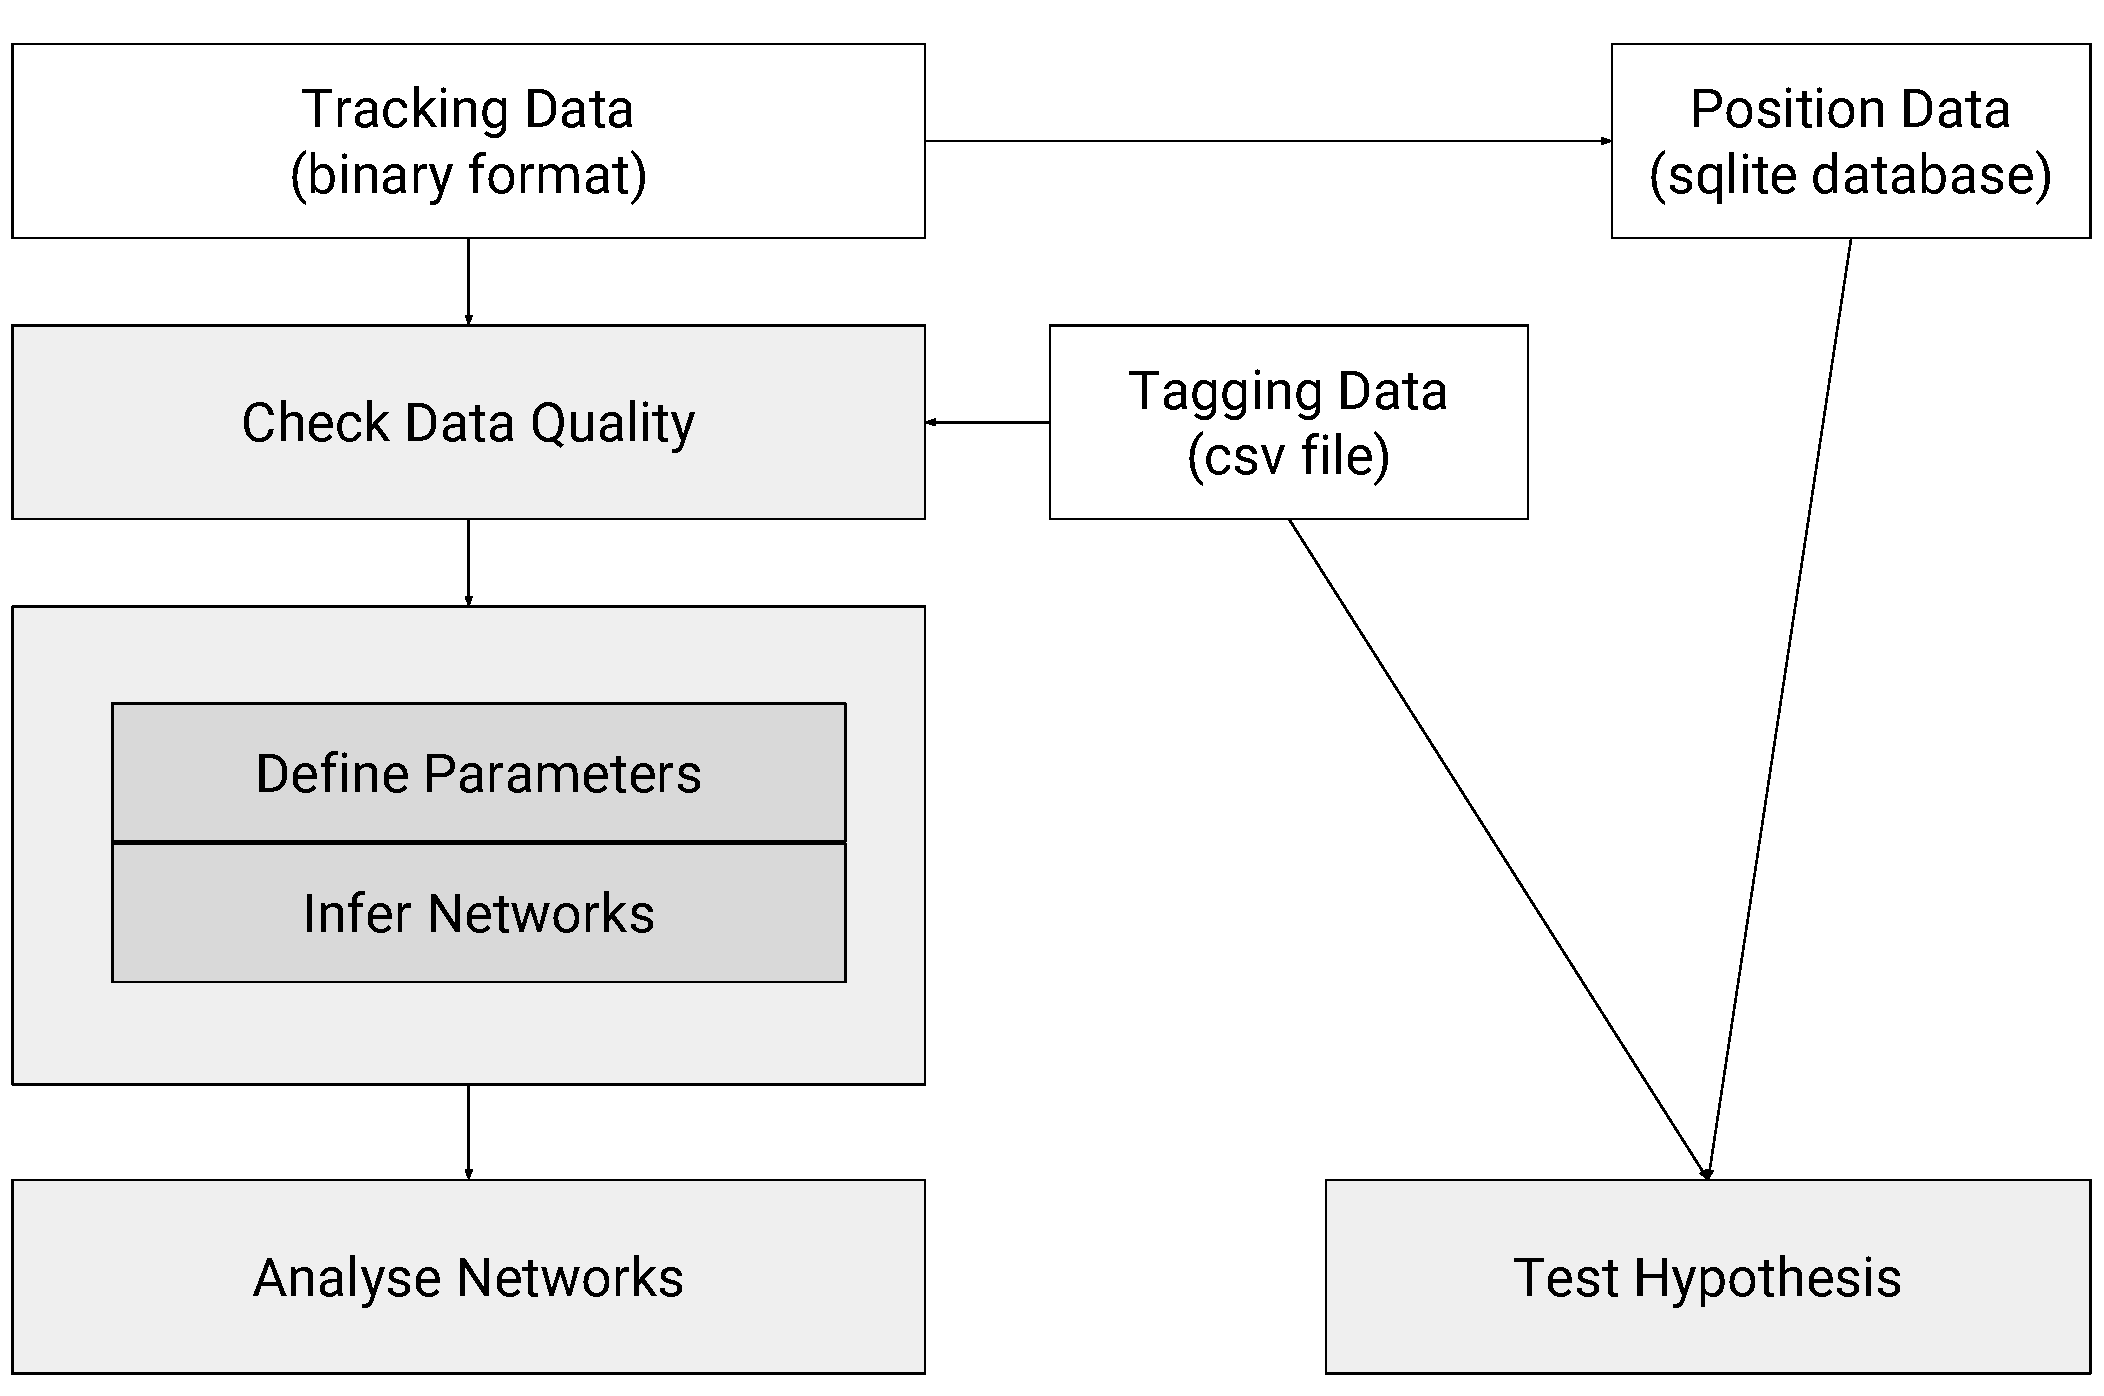
\includegraphics[width=0.8\textwidth]{Figures/process}
	\caption[Steps of the research approach]{\textbf{Steps of the research approach} [TODO: anpassen, iterationen, hypothesis raus, evtl. so viele Schritte im Bild wie Abschitte im Text, zumindest muss das irgendwie anders.]}
	\label{fig:process}
\end{figure}

%%%%%%%%%%%%%%%%%%%%%%%%%%%%%%%%%%%%%%%%%%%%%%%%%%%%%%%%%%%%%%%%%%%%%%%%%%%%%%%
%%%%%%%%%%%%%%%%%%%%%%%%%%%%%%%%%%%%%%%%%%%%%%%%%%%%%%%%%%%%%%%%%%%%%%%%%%%%%%%
%%%%%%%%%%%%%%%%%%%%%%%%%%%%%%%%%%%%%%%%%%%%%%%%%%%%%%%%%%%%%%%%%%%%%%%%%%%%%%%
%%%%%%%%%%%%%%%%%%%%%%%%%%%%%%%%%%%%%%%%%%%%%%%%%%%%%%%%%%%%%%%%%%%%%%%%%%%%%%%
\section{The Dataset}
\label{sec:dataset}
%%%%%%%%%%%%%%%%%%%%%%%%%%%%%%%%%%%%%%%%%%%%%%%%%%%%%%%%%%%%%%%%%%%%%%%%%%%%%%%
%%%%%%%%%%%%%%%%%%%%%%%%%%%%%%%%%%%%%%%%%%%%%%%%%%%%%%%%%%%%%%%%%%%%%%%%%%%%%%%
%%%%%%%%%%%%%%%%%%%%%%%%%%%%%%%%%%%%%%%%%%%%%%%%%%%%%%%%%%%%%%%%%%%%%%%%%%%%%%%
%%%%%%%%%%%%%%%%%%%%%%%%%%%%%%%%%%%%%%%%%%%%%%%%%%%%%%%%%%%%%%%%%%%%%%%%%%%%%%%

\begin{figure}
    \centering
    \begin{subfigure}[b]{\textwidth}
	\centering
	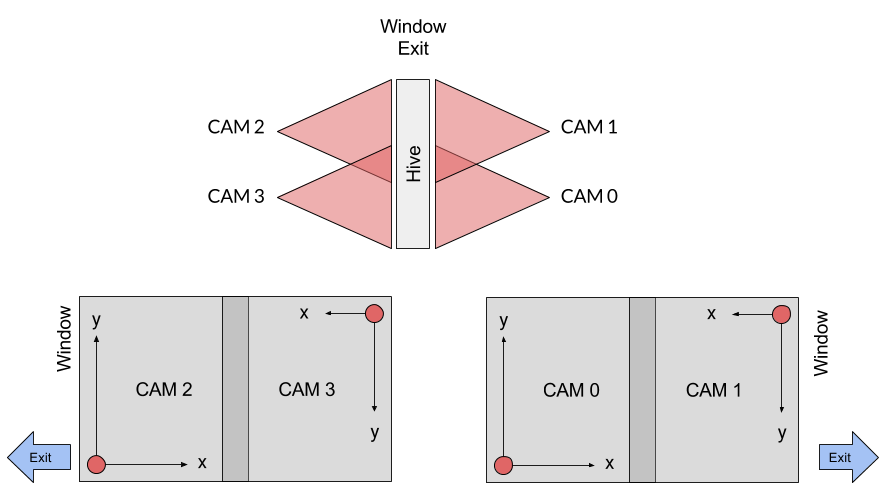
\includegraphics[width=0.8\textwidth]{Figures/setupCams}
	\caption[Camera setup]{\textbf{Camera setup} Each side of the honeycomb is filmed by two cameras. The two cameras per side overlap, bees inside this area are detected from both cameras.}
	\label{fig:cams}
	\vspace{5mm}
    \end{subfigure}
    \begin{subfigure}[b]{\textwidth}
	\centering
	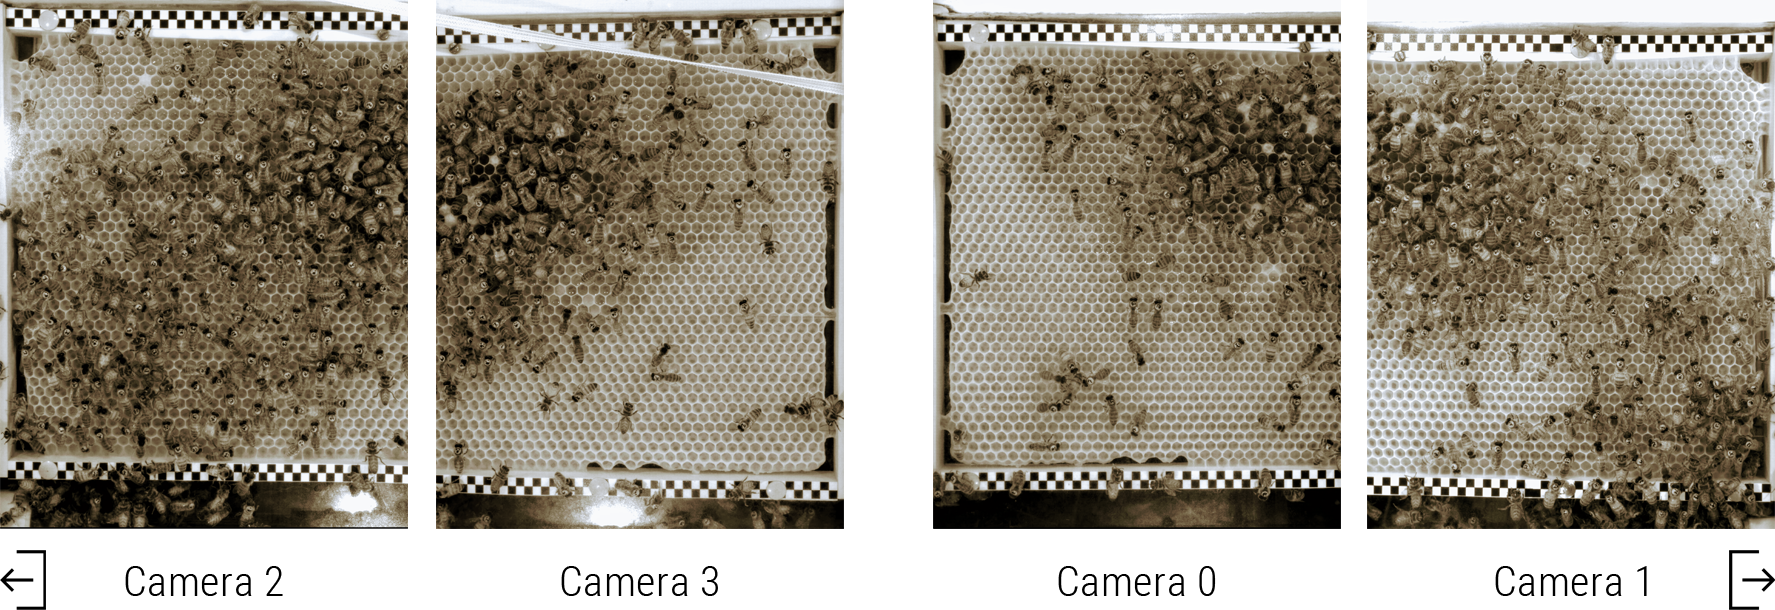
\includegraphics[width=0.65\textwidth]{Figures/beesClose}
	\vspace{5mm}
	\caption[Images for each camera]{\textbf{Images for each camera} Top: side~A, bottom: side~B}
	\label{fig:veryclose}
    \end{subfigure}
 	\caption[Observation setup]{\textbf{Observation setup}}
 	\label{fig:obssetup}
\end{figure}

The dataset derives from high resoluted video files, that capture tagged honey bees of one colony in an single-frame observation hive.
The colony includes about 3200 bees over a period of nine weeks. The bees are uniquely tagged with circular 12-bit markers (figure~\ref{fig:markers}, section~\ref{ch:intro}).
Two cameras per side filmed the complete honeycomb permanently.
Figure~\ref{fig:cams} illustrates the camera setup.
The \emph{recording period} lasted nine weeks (63 days), from 19.07.2016 until 19.09.2016, with some interruptions due to maintenance work and technical failures. An overview about the complete reocrding period is given in figure~\ref{fig:observation-period} in appendix~\ref{ch:appendix}.

All four cameras, each with a resolution of $4000\times3000$ pixels, record $3.5$ frames per second. 
An image analysis pipeline~\cite{wario2015automatic} detects all bees in each frame.
The resulting detection data is stored in a binary file format.
An python library\footnote{The library is called \texttt{bb-binary} and is created by the Biorobotics Lab. It can be found on GitHub: \url{https://github.com/BioroboticsLab/bb_binary}; Last accessed: 2106-02-16, 04:28PM} provides an frame-level access to those binary files.
The size of the dataset is $470$~GB, about $7.5$~GB of binary data per day.

The 67 days long \emph{tagging period} started on 28.06.2016 and lasted until 02.09.2016, resulting in $3.191$ tagged bees. The young bees, which were raised in a separate incubator, were tagged and then added to the observation hive, about noon each day. Figure~\ref{fig:tagging-period} (Appendix~\ref{ch:appendix}) shows the frequency of tagged bees per day. The hatching day for each bee is documented; therefore the age of each bee at a particular point in time can be calculated.

[TODO: Begruendung des gewaehlten Zeitraumes: Funktionstüchtigkeit und Altersverteilung]
For further analysis, I chose three days: 20., 22., and 24. August.

\clearpage
%%%%%%%%%%%%%%%%%%%%%%%%%%%%%%%%%%%%%%%%%%%%%%%%%%%%%%%%%%%%%%%%%%%%%%%%%%%%%%%
%%%%%%%%%%%%%%%%%%%%%%%%%%%%%%%%%%%%%%%%%%%%%%%%%%%%%%%%%%%%%%%%%%%%%%%%%%%%%%%
\subsection{Data Scheme}
\label{subsec:datascheme}
%%%%%%%%%%%%%%%%%%%%%%%%%%%%%%%%%%%%%%%%%%%%%%%%%%%%%%%%%%%%%%%%%%%%%%%%%%%%%%%
%%%%%%%%%%%%%%%%%%%%%%%%%%%%%%%%%%%%%%%%%%%%%%%%%%%%%%%%%%%%%%%%%%%%%%%%%%%%%%%

\begin{table}[!t]
\colorbox{usethiscolorhere}{
\centering
\begin{tabularx}{\textwidth}{@{} r Y @{}}
	\textbf{Frame container} &
	A container for all frames, which belong to a specific video file of a certain camera.\\
	\textbf{Frame} &
	This includes all detections of one camera image at a certain point in time.\\
	\textbf{Detection} &
	A detection of a bee at a certain point in time.\\
	\textbf{Decoded ID} &
	Identifier of a bee consisting of 12 probability values, representing 12 bits.\\
	\textbf{Confidence} &
	Value between 0\% and 100\%.\\
	\textbf{ID} &
	The decimal representation of an decoded ID, after applying a certain confidence value.\\
	\textbf{Bee time series} & Binary sequence, indicating the absence and presence of a certain bee in a particular time interval.\\
	\textbf{Pair time series} & Binary sequence, indicating the absence and presence of two bees in a particular time interval.\\
\end{tabularx}
}
\end{table}

The data is organized in so-called \emph{frame containers}.
Each frame container corresponds to one video file of a single camera and consists of about $1024$ \emph{frames}. So the frame container specifies the camera (\emph{camId}), which recorded the video.
Each frame holds a list of bees, which were detected by the image analysis pipeline and is attributed with a \emph{timestamp}.

A bee \emph{detection} has, among others, the following attributes:

\begin{table}[!h]
\centering
\begin{tabular}{rl}
\textbf{xpos}: & $x$ coordinate of bee with respect to the image in pixel \\
\textbf{ypos}: & $y$ coordinate of bee with respect to the image in pixel \\
\textbf{decoded ID}: & decoded 12-bit ID \\
\textbf{cam ID}: & ID of the camera ${0,1,2,3}$ \\
\textbf{timestamp}: & unix timestamp with milliseconds\\
\end{tabular}
\end{table}

The data can be accessed by iterating on the frame level, using a start and end time\-stamp for specifying a time interval. The complete data scheme can be found on GitHub\footnote{\url{https://github.com/BioroboticsLab/bb_binary/blob/master/bb_binary/bb_binary_schema.capnp}; Last accessed: 2106-02-16, 04:46PM}. 



%%%%%%%%%%%%%%%%%%%%%%%%%%%%%%%%%%%%%%%%%%%%%%%%%%%%%%%%%%%%%%%%%%%%%%%%%%%%%%%
%%%%%%%%%%%%%%%%%%%%%%%%%%%%%%%%%%%%%%%%%%%%%%%%%%%%%%%%%%%%%%%%%%%%%%%%%%%%%%%
\subsection{ID Probabilities, Confidence Level, and Quality}
\label{subsec:confidence}
%%%%%%%%%%%%%%%%%%%%%%%%%%%%%%%%%%%%%%%%%%%%%%%%%%%%%%%%%%%%%%%%%%%%%%%%%%%%%%%
%%%%%%%%%%%%%%%%%%%%%%%%%%%%%%%%%%%%%%%%%%%%%%%%%%%%%%%%%%%%%%%%%%%%%%%%%%%%%%%

\begin{figure}
    \centering
    \begin{subfigure}[b]{0.45\textwidth}
        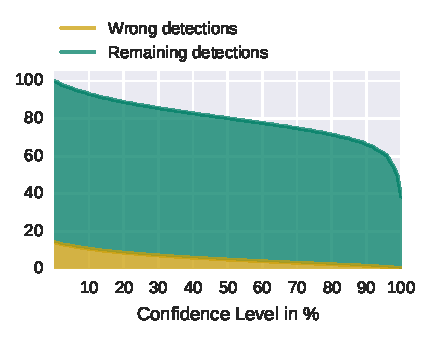
\includegraphics[width=\textwidth]{Figures/detectionsWrongConf}
        \caption[Detections]{\textbf{Detections}}
        \label{fig:detections}
    \end{subfigure}
    \begin{subfigure}[b]{0.45\textwidth}
        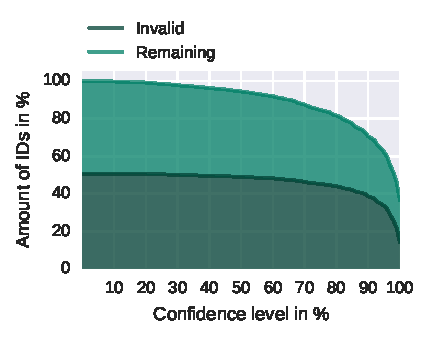
\includegraphics[width=\textwidth]{Figures/idsWrongConf}
        \caption[IDs]{\textbf{IDs}}
        \label{fig:ids}
    \end{subfigure}
 	\caption[Quality of detections and IDs]{\textbf{Quality of detections and IDs} \emph{Green} represents the number of remaining detections and remaining IDs (from $4096$ possible IDs). \emph{Yellow} indicates the fraction of wrong IDs and wrong detections in relation the remaining number of IDs and detections.\protect\footnotemark}
 	\label{fig:remainingVSquality}
\end{figure}

\footnotetext{Data set: 26.07.2016, 4~p.~m., 10~minutes, all cameras}

Twelve bits can encode the identity of 4096 bees.
Each bit of the decoded ID is not a one or zero but represents a probability between $0$ and $255$, normalized to a value between $0$ and $1$.
Therefore, a bit indicates the confidence of the image analysis pipeline for that specific bit.
I define the confidence $c$ for a bit $b$, analogously to Leon~\textcite[p.~14]{leon2016}, as $c(b)=2\cdot|b-0.5|$.
The confidence of a decoded ID is, accordingly, the minimum of all twelve bits' confidences.
Consequently, a high level of confidence reduces the amount of data, which remains for further processing.

I use the age information of the bees to check the quality of the remaining data.
The age is specified in days.
An age of $0$ days indicates that a bee was born on that day.
It is possible that the resulting age is below $0$ days.
One the one hand, this happens when the pipeline detected a bee, that was not born yet.
On the contrary, this can happen, if it discovered a bee tag, that was never used during the study, then the age is set to $-100$ days.

I examined (1) the number of detections and (2) the number of unique IDs, depending on the chosen confidence.

For (1) I calculated the age of each bee detection.
A detection with a negative age is counted as a \emph{wrong detection}.
I assumed that a similar number of wrong detections also occurred among detections with a positive age, but remained unseen; therefore I doubled the error\footnote{I chose the 26.07.2016 for testing this because half of the bee tags ($2014$ out of $4096$) were already assigned.}.
For (2), analogously a unique ID with a negative age is counted as a \emph{wrong ID}. The total amount of wrong IDs is doubled.

As expected, with increasing confidence, the number of remaining detections and the amount of remaining unique IDs decreased (figure~\ref{fig:remainingVSquality}).
Also even though the number of wrong detections decreases steadily with an increasing confidence level, the number of wrong IDs only starts to decline with a very high level of confidence.
With a confidence level of 100\%, 30.2\% of the remaining unique IDs are invalid, corresponding to only 2.5\% of invalid detections.

Therefore, to obtain a more reliable dataset, invalid detections need to be filtered out, independently of the confidence value.
The amount of data that remains for further processing is still highly dependent on the chosen level of confidence.

%%%%%%%%%%%%%%%%%%%%%%%%%%%%%%%%%%%%%%%%%%%%%%%%%%%%%%%%%%%%%%%%%%%%%%%%%%%%%%%
%%%%%%%%%%%%%%%%%%%%%%%%%%%%%%%%%%%%%%%%%%%%%%%%%%%%%%%%%%%%%%%%%%%%%%%%%%%%%%%
\subsection{Time Series of Bees and Bee Pairs}
\label{subsec:tracking}
%%%%%%%%%%%%%%%%%%%%%%%%%%%%%%%%%%%%%%%%%%%%%%%%%%%%%%%%%%%%%%%%%%%%%%%%%%%%%%%
%%%%%%%%%%%%%%%%%%%%%%%%%%%%%%%%%%%%%%%%%%%%%%%%%%%%%%%%%%%%%%%%%%%%%%%%%%%%%%%

The dataset, is transformed to binary \emph{bee time series}, depicted in figure~\ref{fig:structure} (left and middle). A time series of a bee is a sequence of zeros and ones indicating the absence and presence of a bee over a specified time interval. 
I examined the effect the level of confidence has on the bee time series.
As expected, with an increasing confidence level the average gap length decreases and the overall number of gaps increases (figure~\ref{fig:gaps}).

The number of gaps, those bee time series has, is important because in a later step I want to extract pairs of close bees, who are present at the very same time. I call those \emph{pair time series}, as shown in figure~\ref{fig:structure} (right). So a lot of gaps in bee time series could lead to a lot of gaps in the pair time series.

\begin{figure}[htb]
	\centering
	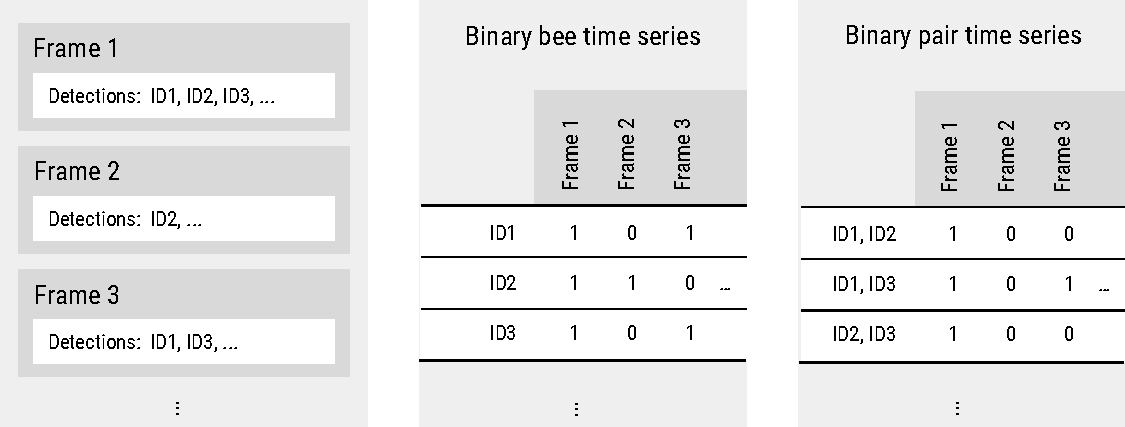
\includegraphics[width=1.0\textwidth]{Figures/structure}
	\caption[Structure of dataset]{\textbf{Structure of dataset} \emph{Left}: original dataset - containing a sequence of frames with bee detections; \emph{Middle:} binary bee time series - zero and one indicate absence and presence of a bee; \emph{Right:} binary pairs time series - zero and one indicate the absence and presence of two bees in the same frame.}
	\label{fig:structure}
\end{figure}

\begin{figure}[htb]
	\centering
	\begin{subfigure}[b]{0.45\textwidth}
		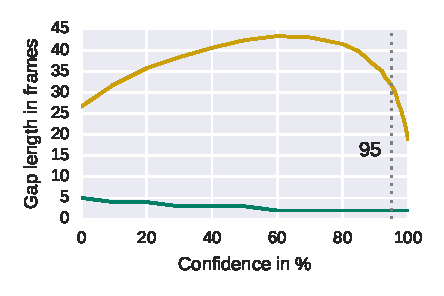
\includegraphics[width=\textwidth]{Figures/gaplen}
		\caption[Length of gaps]{\textbf{Length of gaps}}
		\label{fig:gaplen}
	\end{subfigure}
	\begin{subfigure}[b]{0.45\textwidth}
		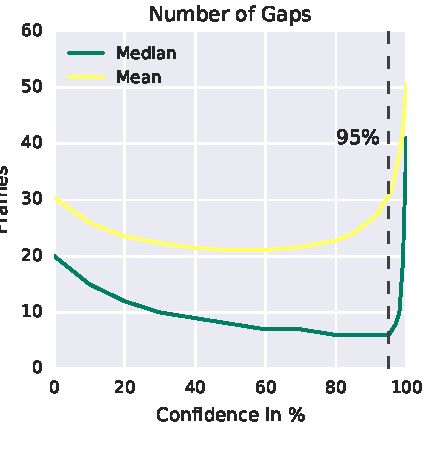
\includegraphics[width=\textwidth]{Figures/numgaps}
		\caption[Number of gaps]{\textbf{Number of gaps}}
		\label{fig:numgaps}
	\end{subfigure}
	\caption[Influence of Confidence Level on Gaps]{\textbf{Influence of confidence level on gaps} [TODO: add legend][TODO:gaps D] With an increasing level of confidence the average gap length decreases and the number of gaps per bee series increases. \emph{Orange} indicates the median, \emph{green the mean}.\protect\footnotemark }
	\label{fig:gaps}
\end{figure}

\footnotetext{Data set: 26.07.2016, 16:00-16:05}


%%%%%%%%%%%%%%%%%%%%%%%%%%%%%%%%%%%%%%%%%%%%%%%%%%%%%%%%%%%%%%%%%%%%%%%%%%%%%%%
%%%%%%%%%%%%%%%%%%%%%%%%%%%%%%%%%%%%%%%%%%%%%%%%%%%%%%%%%%%%%%%%%%%%%%%%%%%%%%%
\subsection{Detection Frequency Filter}
%%%%%%%%%%%%%%%%%%%%%%%%%%%%%%%%%%%%%%%%%%%%%%%%%%%%%%%%%%%%%%%%%%%%%%%%%%%%%%%
%%%%%%%%%%%%%%%%%%%%%%%%%%%%%%%%%%%%%%%%%%%%%%%%%%%%%%%%%%%%%%%%%%%%%%%%%%%%%%%
A good indicator, whether a bee is alive and present on a particular day, is its detection frequency. The hypothesis is: Bees who have a low detection rate are not physically present in the hive, respectively do not exists at that day.
To check this hypothesis, I investigate whether there is a correlation between the age of bees and their detection frequency.

\begin{figure}[t]
	\centering
	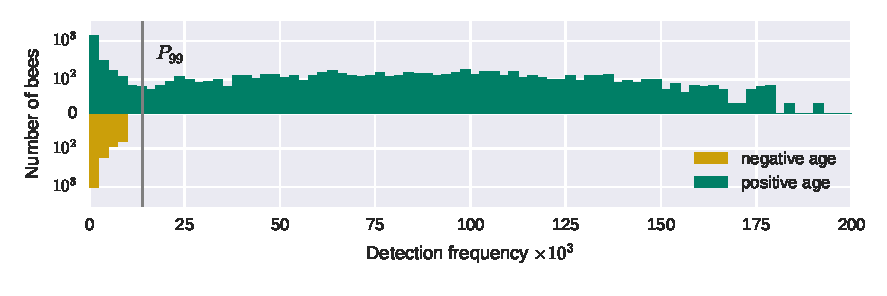
\includegraphics[width=1.0\textwidth]{Figures/filter}
	\caption[Detection frequency of IDs]{\textbf{Detection frequency of IDs} [TODO: add legend] \emph{Orange} coressponds to bees with a negative age and \emph{green} displays bees with a positive age.\protect\footnotemark}
	\label{fig:filter}
\end{figure}

\footnotetext{Data set: 20.08.2016, 24 hours, number of total frames: 302400}

Bess with a negative age are on average detected less frequently than bees with a positive age.
In advance, I excluded bees from the statistics, which had a negative age, but a detection frequency over 10000 frames. Their detection frequency is similar to that from bees with a positive age. I looked at the corresponding photos taken by the camera and confirmed that those are living bees and no artifacts.\footnote{Probably a mistake in the table, which reports the hatching days for each bee.}
Also I excluded bees~($n=10$), whose age is unknown\footnote{id= [2,
    74,
    2045,
    3172,
    3764,
    3796,
    3827,
    3836,
    3844,
    3940]}.

For each analysis day, the number of detections per ID is obtained, excluding the mentioned IDs.
Additionally, I discarded all detections with an ID frequency below the 99th percentile of negative IDs.
A list of valid IDs per day is kept to filter out wrong detections beforehand.

%%%%%%%%%%%%%%%%%%%%%%%%%%%%%%%%%%%%%%%%%%%%%%%%%%%%%%%%%%%%%%%%%%%%%%%%%%%%%%%
%%%%%%%%%%%%%%%%%%%%%%%%%%%%%%%%%%%%%%%%%%%%%%%%%%%%%%%%%%%%%%%%%%%%%%%%%%%%%%%
\subsection{Implications}
%%%%%%%%%%%%%%%%%%%%%%%%%%%%%%%%%%%%%%%%%%%%%%%%%%%%%%%%%%%%%%%%%%%%%%%%%%%%%%%
%%%%%%%%%%%%%%%%%%%%%%%%%%%%%%%%%%%%%%%%%%%%%%%%%%%%%%%%%%%%%%%%%%%%%%%%%%%%%%%
The confidence level is set to 95\%.
This a good balance between gaps in the time series and quality of the data and amount of remaining data.
Because bee time series contain a lot of short gaps (mean = 3, 95\% confidence), the inference of edges (bees that are spatially close to each other at the same time), should take this into account.

\clearpage
\section{Inferring Networks}

The following part describes the pipeline for generating spatial proximity networks out of honey bee tracking data. A node in the network is a bee. They are distinguished by IDs. Only bees are in the network who interact at least once with another bee.

undirected and weighted, aggregated networks\\

Two bees are associated (spatially close to each other), if their distance is minor to a \emph{maximum distance}. As everything is very close in a bee hive this value is hard to choose. Only this criteria is very week, meaning having a resolution of three frames per seconds results in interactions which could only last for $0.33$ seconds. So an additional parameter the \emph{minimum contact duration} is introduced, it is the minimum time they have to spend at least nearby to be called associated.

Taking the fragmentation of tracks into account, it is obvious that two bees could be nearby but not at the very same time, but slightly shifted. So the minimum contact duration would be too errow prone. To overcome this issue one could correct the bee tracks, by filling gaps of varius sizes and interpolating the position of that bee accordingly. This is rather time consuming for this amount of tracking data (TODO: naja so doll auch nicht) and also considering, that the tracking data is going to be improved in the future, then manipulating the raw data seems senseless. I rather perform a gap filling (maybe similar to binary dilation?) on the time series of pairs, but not on the bee tracks, because this is independent of the input data.

Edges are attributed with two parameters. The first one is the frequency of contacts, so how often they share a close position. The second parameter is the total duration of contact, how many time frames in total they spend close by.

\subsection{Network Pipeline}

The network pipeline takes as input a path to the bb-binary data and outputs a graph in graphML file format. The pipeline takes the following parameters:

\begin{itemize}
\item path to data
\item confidence in percent
\item gap size in frames - this is used to corret the time series of bee pairs
\item maximum distance in px - define what close means (spatial proximity)
\item minimum contact duration in frames - how many frames bees need to spend nearby
\item cutoff in percent - IDs with a number of total detections below X percent of the mean frequency are discarded 
\item start timestamp - start of network slice
\item window size in minutes - size of time window for aggregating the network
\item number of used CPUs for parallelization
\item year - calculate IDs and set camera setup for 2015 or 2016
\end{itemize}

The pipeline is parallelized on frame level, that means, each process gets a portion (frames for a timeinterval of five minutes) of the data and extracts interactions/edges. The main process adds everything up and creates a network.
The steps are the following:

\begin{enumerate}
\item \textbf{Filter detections by confidence}\\
For each of the four camera the detections are filtered by the confidence level.

\item \textbf{Simple stitching}\\
Each side of the hive consists of two cameras. 	The $x$-coordinates of each detection (of the right	cameras) is moved further to the right, also adding an offset of $2\times \texttt{maximum distance}$. So the left and the right detection of each side of the hive are move into one reference system.

\item \textbf{Syncronize Cameras}\\
For each side of the hive the cameras need to be syncronized. In the normal case the difference between consecutive frames should be about $0.332$~seconds, due to technical problem this value can be lower ($0.003$ ) and higher ($2.932$) at certain times. Cameras 3 and 2 and cameras 1 and 0 are matched, frames without a match are dropped (shorter number of frames, matchen, threshold $0.33/2$, minimum).

\item \textbf{Discard Detections with certain IDs}\\
All detections whos ID is in a list are keept, other detections are discarded. (see frequency filter)

\item \textbf{Extract close pairs}\\
For each side of the hive, all close pairs according to the maximum distance parameter are calculated and then joined together.

\item \textbf{Generate time series of bee pairs}\\
The data structure (frames and detection) is transformed to time series of bee pairs.

\item \textbf{Correct pair time series.}\\
The time series of bees are corrected by filling in the gaps of length \texttt{gap size}.

\item \textbf{Extract edges}\\
The edges and its attributes (frequency and duration) are extracted from the time series of bees using the minimum contact duration parameter. A sequence of at least X ones counts as one interaction. The frequency of those series adn the total duration (number of ones) are the attributes.


\end{enumerate}

\subsection{Pipeline Parameters}
For performing the network analysis, I chose the pipeline parameters as follows:

\begin{description}
\item[Confidence] As explained in section\ref{subsec:confidence}, the confidence is set to $95\%$.

\item[Maximum Distance] I chose the length of a bee body, according to \textcite{baracchi2014socio}, as the maximum distance between two bees (figure~\ref{fig:radius}). The average bee length of $212$px ($\pm 16$px)  was determinded by manually measuring the length of all bees ($n=337$) in four images (one for each camera, 21.07.2016, 03:00PM) using the tool ImageJ\footnote{\url{http://imagej.net/Welcome}; Last accessed: 22.02.2016}.

\item[Gap Size] The gap size is set to two frames. This value corresponds to the median gap length in the time series of pairs ($\texttt{mode}=1$, $\texttt{mean}=27$). [TODO: what dataset was used (95\% confidence, XXX\% cutOff, XXXpx maximal distance, date, camera)]

\item[Minimum Contact Duration] This is set to three frames (one second). This corresponds to~\textcite{mersch2013tracking}, they as well exclude interactions below one second. Looking at the frequency distribution of chains of ones ($1$, $11$, $111$, and so on) of the pair time series (after filling the gaps), then: $\texttt{mode}=1$, $\texttt{median}=2$ and $\texttt{mean}=4$. Three frames corresponds to $57\%$ of all chains, this seem to be reasonable. [TODO: what dataset was used (95\% confidence, XXX\% cutOff, XXXpx maximal distance, date, camera)]

\end{description}

\begin{figure}[htb]
	\centering
	\begin{subfigure}[b]{0.4\textwidth}
		\centering
		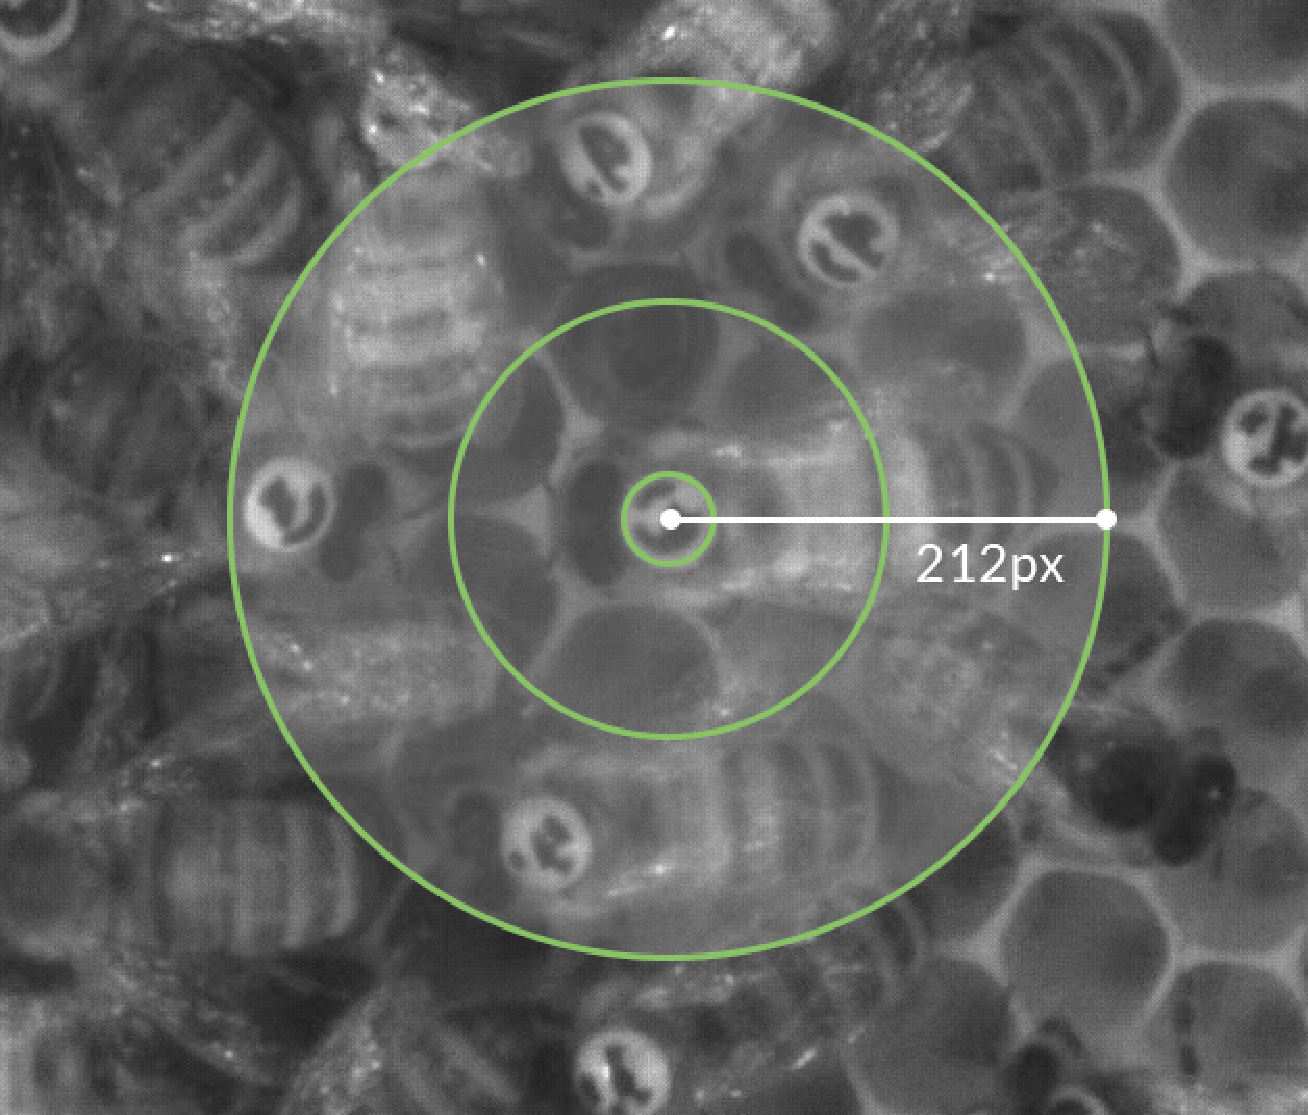
\includegraphics[width=\textwidth]{Figures/radius}
		\caption[Contact Radius]{Contact Radius}
		\label{fig:radius}
	\end{subfigure}
	\begin{subfigure}[b]{0.4\textwidth}
		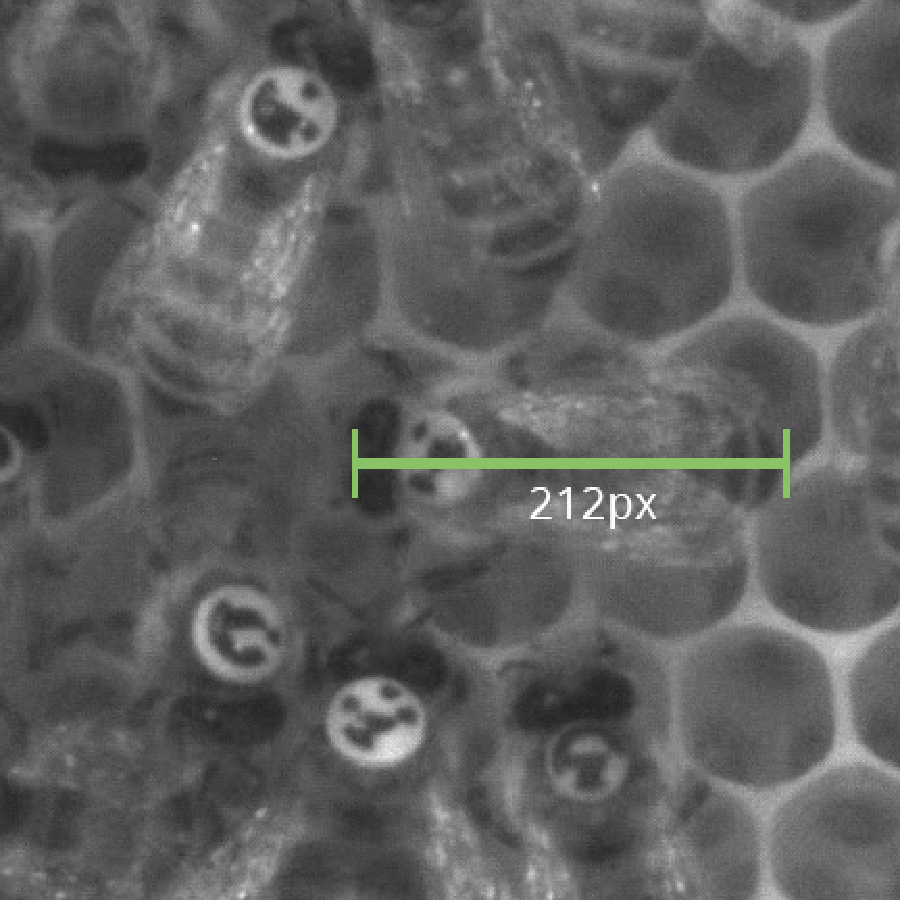
\includegraphics[width=\textwidth]{Figures/sizeTagBee}
		\caption[Bee and Tag Size]{Bee Length}
		\label{fig:size}
	\end{subfigure}
	\caption{Distance Between Bees: A length of a bee is chosen as the maximal  distance between bees.}
	\label{fig:contactRadius}
\end{figure}

\clearpage
\section{Static and Temporal Analysis}

Despite the possibility of generating networks of different granularity (resolution is minutes), here for further analysis daily networks (10h, two hours after sunrise until zwo hours before sunset) are aggregated.


\textcite{wey2008social}

\subsection{Static Network Analysis}
The following network properties were analysed for a static day and hour network.\\
TODO: list of properties. (similar to what others have done)
nodes, edges, density, diameter\\


\subsection{Temporal Analysis}
three day networks (2 days gap)\\
one network 2 weeks later\\

\subsection{Community Detection}
I tested all community detection algorithms implemented in python, to find an algorithm, which works well for my case of animal social networks. The three most common python libraries for network analysis were reviewed: NetworkX\footnote{\url{https://networkx.github.io/}; Last accessed: 16.03.2016, 6:36~p.m.}, igraph\footnote{\url{http://igraph.org/python/}; Last accessed: 16.03.2016, 6:38~p.m.}, and graph-tool\footnote{\url{https://graph-tool.skewed.de/}; Last accessed: 16:03.2016, 6:39~p.m.})

The algorithm needs to fulfill the following criteria:

\begin{itemize}
\item Support for large and very dense networks ($N>1000$, $D>50~\%$)
\item Support weighted edges
\item Fast runtime
\end{itemize}

Table~\ref{tab:algos} gives an overview about the twelve algorithms reviewed. Five algorithms did not terminate after 15~minutes and were therefore excluded from further investigations. Infomap and label propagation tend to partition all nodes into a single community, this is known especially in dense graphs~\cite{yang2016comparative, fortunato2010community}.
The Louvain algorithm is the same as multilevel, but takes longer producing almost the same communities and therefore was also excluded. Walktrap was tested for different step size parameters, as suggested in~\cite{pons2005computing}, the communities remained almost the same (only a few nodes switched communities). 

I had a closer look at fastgreedy, leading eigenvector, multilevel, and walktrap regarding the number of detected communities and community size for all three networks. Table~\ref{tab:algos4} shows the results. All algorithms found at least two communities. Except for leading eigenvector, there is a tendency that a third community exists.
I decided to use two algorithms for community detection: leading eigenvector and walktrap. \textcite{farine2015constructing} explains that leading eigenvector is often used with animal social networks and works well. Walktrap is chosen for also  examining the possible third community.

There are comparative analysis of community detection algorithms, e.g.~\cite{yang2016comparative, harenberg2014community}. They seem to be promising, but assume eighter a power law degree distribution or evaluate networks with a low density, which is not applicable here.

\begin{table}[htbp]
\small
\caption[Compairing community detection algorithms]{\textbf{Comparing community detection algorithms} Comparison of algorithms implemented in python. Criterias are the support of weighted edges, runtime and number of communities. A runtime indicated by $-$ mean no termination after 15~minutes.\\
}
\label{tab:algos}

\begin{tabularx}{\textwidth}{lcccccccccccc}
\toprule
	 {} &
	 \rotatebox{90}{\textbf{fastgreedy$^1$}} &
	 \rotatebox{90}{\textbf{leading eigenvector$^1$}} &
	 \rotatebox{90}{louvain$^2$} &
	 \rotatebox{90}{\textbf{multilevel$^1$}} &
	 \rotatebox{90}{\textbf{walktrap$^1$}} &
	 
	 \rotatebox{90}{infomap$^1$} &
	 \rotatebox{90}{label propagation$^1$} &
	 
	 \rotatebox{90}{edge betweenness$^1$} &
	 \rotatebox{90}{k-clique communities$^2$\thinspace} &
	 \rotatebox{90}{optimal modularity$^1$} &
	 \rotatebox{90}{spinglass$^1$} &
	 \rotatebox{90}{statistical inference$^3$} \\ \midrule
	 
	 
	 
	 Edge weights & $\times$ & $\times$ & $\times$ & $\times$ & $\times$ & $\times$ & $\times$ & & $\times$ & $\times$ & $\times$ \\ \midrule
	 Runtime in sec & ~$3.6$ & ~$6.3$ & $11.7$ & ~$0.7$ & $19.4$ & $13.2$ & ~$0.2$ & $-$ & $-$ & $-$ & $-$ & $-$ \\ \midrule
	 Communities & $3$ & $2$ & $2$ & $3$ & $2$ & $1$ & $1$ & $-$ & $-$ & $-$ & $-$ & $-$ \\ \midrule
	  & 473 & 488 & 469 & 462 & 490 & 922 &  922 &  &  &  &  &  \\
	  & 434 & 434 & 453 & 427 & 431 &  &  &  &  &  &  &  \\
	  & 15 &  &  & 33 & (1) &  &  &  &  &  &  &  \\
	 \bottomrule
	 
\end{tabularx}
\begin{flushright}
\footnotesize{
$^1$ igraph, $^2$ NetworkX, $^3$ graph-tool\\
}
\end{flushright}

\end{table}

% \hdashline
% \midrule
% \bottomrule
\begin{table}[htbp]
\centering
\caption[X]{\textbf{X} X\\
}
\label{tab:algos4}

\begin{tabular}{lcccc}
\toprule
	 {} &
	 fastgreedy &
	 leading eigenvector &
	 multilevel &
	 walktrap \\ \midrule
	 
	  Network 1
	  & 473 & 488 & 462 & 490 \\
	  & 434 & 434 & 427 & 431 \\
	  & 15 &   & 33 & (1) \\ \midrule
	  Network 2
	  & 504 & 503 & 481 & 372 \\
	  & 467 & 475 & 439 & 311 \\
	  & 7 &   &  58 & 294 \\
	  & & & & (1) \\ \midrule
	  Network 3
	  & 534 & 537 & 505 & 310 \\
	  & 388 & 385 & 415 & 390 \\
	  &  &   &  (2) & 231 \\
	 \bottomrule
	 
\end{tabular}

\end{table}

% \hdashline
% \midrule
% \bottomrule

\section{Attributed Data and Hypothesis Testing}
Hypothesis\\
(1) Communities reflect groups of bees working in different areas of the hive and\\
(2) Communities reflect different age groups\\

The data which was used to test the hypothesis (1) is saved in a sqlite database for faster access, because using bb\_binary (parsing the data over and over again) was to slow. For testing if lists of positions (spatial ditribution) are different the test XY was used [TODO: what to use here]

For hypothesis (2) the data is stored as a csv file of birth dates of each bee. For testing if age goups are different the Kolmogorov Smirnov Test was used.
\section{Implementation, Runtime and Complexity}
For implementing the network pipeline python, with pandas and numpy, are used, because the bb\_binary library, for accessing the tracking, data is only available in python. The networks, in graphML format, are created using the python library \emph{NetworkX}\footnote{\url{https://networkx.github.io/} ; Last accessed: 2017-02-17, 08:07PM} in version 1.11.
I used iGraph for community detection. Some bash scrips for generating multiple networks.

Bottleneck is reading bb\_binary data into pandas dataframes.
i used the multithreading for distributing the data an alevel of 5 minutes (a process the frames coresponding to 5 minutes).

Maybe some table with how long what step needs, with how many cores (hom much RAM and so on).
\chapter{Results}

I analysed three daily networks, these are refererred to below as \#1, \#2, and \#3. Each network is aggregated for ten hours starting at 8~a.m. and lasting until 6~p.m. I chose the 20.08.2016, 22.08.2016, and 24.08.2016, because at this point in time the hive also contained tagged foragers (older bees). At the same time young bees were added to the colony (see table~\ref{tab:networks} for details). The age distribution for each network is shown in figure~\ref{fig:ages}.

[TODO: PLOT How many nodes in the network stay the same over 3 timesteps? (will be going next step, same, new ones)]

\begin{table}
\centering
\begin{tabular}{ccccccc}
\toprule
{} & 20.08.16 & 21.08.16 & 22.08.16 & 23.08.16 & 24.08.16 \\
\midrule
Network ID & \#1 & - & \#2 & - & \#3 & \\
Number of added bees & 0 & 0 & 110 & 60 & 0 \\
Time added & - & - & 2~p.m. & 6~p.m. & - \\
\bottomrule
\end{tabular}
\caption[TODO]{Overview about networks and number of added bees.}
\label{tab:networks}
\end{table}

\begin{figure}[htb]
	\centering
	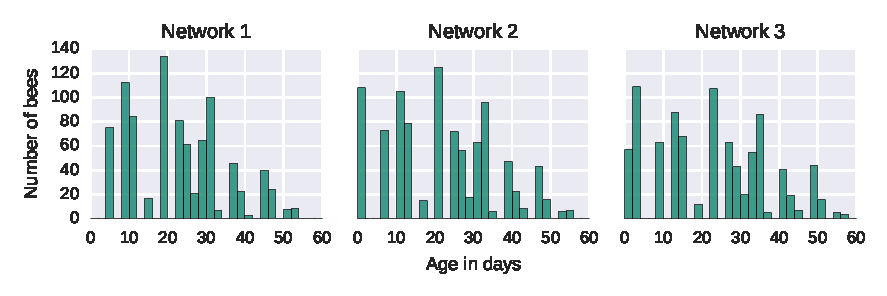
\includegraphics[width=1.0\textwidth]{Figures/ages}
	\caption[Age distribution per network]{Age distribution per network: The width of a bar corresponds to two days.}
	\label{fig:ages}
\end{figure}

\section{Network type and properties}
 
\subsection{Global Structure - Network Level}
Each network consists of one giant component. Table~\ref{tab:stats} summarizes basic network properties number of nodes, number of links, density, diameter, average shortest path length, global clustering coefficient, average degree, and average strength.\\

TODO: high density, small diameter, very short average path length, high clustering coefficient, high strength and degree, compared to what? random graph\\

TODO: calc network centralisation and add to table\\
TODO: PLOT degree and strength distribution\\
TODO: PLOT edge weight distribution\\

\begin{table}
\centering
\begin{tabular}{lcccccccc}
\toprule
{} &  $N$ &   $L$ &  $D$ &  $\langle d_{\texttt{max}} \rangle$ &  $\langle d \rangle$ &   $C_\Delta$ &  $\langle k \rangle$ &  $\langle s \rangle$ \\
\midrule
\#1 &    922 &  291179 &     0.69 &         3 &              1.32 &  0.79 &      631.62 &      5680.17 \\
\#2 &    978 &  256066 &     0.54 &         3 &              1.46 &  0.72 &      523.65 &      3977.94 \\
\#3 &    922 &  259421 &     0.61 &         3 &              1.39 &  0.75 &      562.74 &      4205.99 \\
\bottomrule
\end{tabular}
\caption[Global network properties]{Global network properties}
\label{tab:stats}
\end{table}

\subsection{Local Structure - Node Level}

[TODO: PLOT closeness, betweenness, local clustering coefficient, eigenvector centrality, weighted and unweighted]

\subsection{Network type}

[TODO: compare to random graph]\\
degree distribution random poisson or binominal, not random power law\\
giant component, connectedness\\
average path length and diameter very small, small world phenomenon\\
higher clustering coefficient than in random\\

\section{Network Metrics in Relation to Age of Bees}

[TODO: all plot in relation to age]

\section{Community Detection}

TODO: if time: show that communities are robust in terms of ilen and radius\\
TODO: age: müsste man eigentlich nochmal gegen ein randomisiertes Modell testen. Alter randomisieren\\

Using the leading eigenvector community detection algorithm revealed in all three networks two communities with about the same number of nodes. The exact number of community members is shown in table~\ref{tab:networks}. The first community contains the queen and bees who are on average younger than the second community. The age difference for network 1 is $8.4$ days, for network 2 $10.9$ days, and for network 3 $14.4$ days on average. The age distribution for each community and network is depicted in figure~\ref{fig:ageDistribution}.

A two sample Kolmogorov–Smirnov test showed, that for each network, the age distributions are significantly different ($p=1.7e^{-32} \pm2.9e^{-32}$).

\begin{table}
\centering
\begin{tabular}{ccrrr}
	\toprule
	{}  & Number of members & Proportion & Age & SD\\
	\midrule 
	\#1  & 488     & 52.93\% & $25.15$ & $\pm19.49$ \\
	             & $434^*$ & 47.07\% & $16.81$ & $\pm17.91$ \\
	\midrule   							
	\#2  & $503^*$ & 51.43\% & $15.44$ & $\pm19.54$ \\
	             & 475     & 48.57\% & $26.37$ & $\pm18.01$ \\
	\midrule  
	\#3  & 537     & 58.24\% & $27.26$ & $\pm17.84$ \\
	             & $385^*$ & 41.76\% & $12.85$ & $\pm20.24$ \\
	\bottomrule
\end{tabular}
\caption[Overview about communities]{Overview about communities per network: Communities marked with * contain the queen.}
\label{tab:communities}
\end{table}

\begin{figure}[htb]
	\centering
	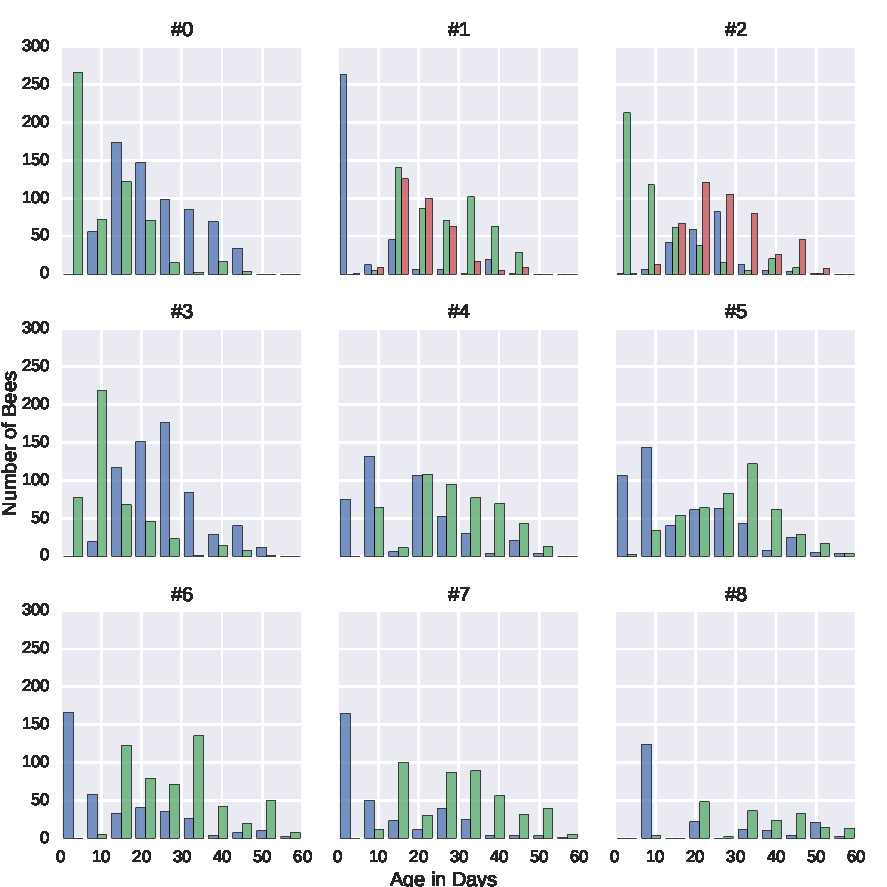
\includegraphics[width=1.0\textwidth]{Figures/ageDistribution}
	\caption[Age distribution for each community and network] {Age distribution for each community and network: The \emph{blue} bar is the community containing the queen. The queens age is not included in the statistic. The \emph{green} bars coresspond to the second community, containing older bees.}
	\label{fig:ageDistribution}
\end{figure}

The younger community spends most time in the center of the comb. The older group is situated on the outer parts, this is the same for all 3 networks. This suggest stable communities in termns of age and spatial distribution.

\begin{figure}[b]
	\centering
	\begin{subfigure}[b]{1.0\textwidth}
		\centering
		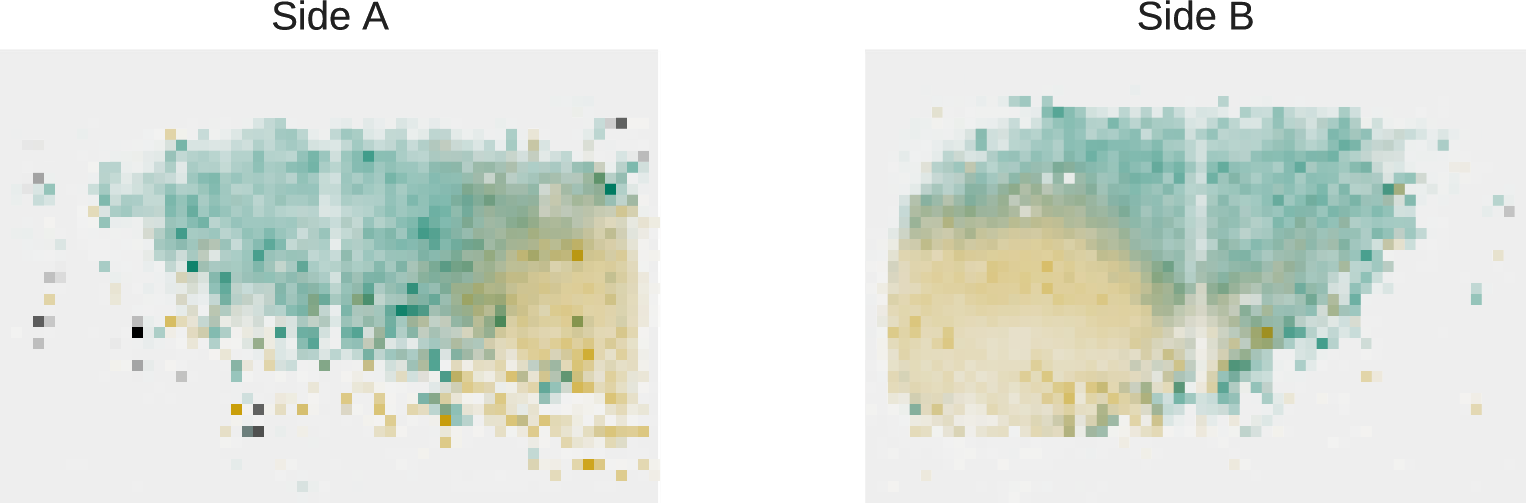
\includegraphics[width=\textwidth]{Figures/network1}
		\caption[Network 1]{Network 1}
		\label{fig:n1}
		\vspace*{5mm}
	\end{subfigure}
	%\vspace{1cm} 
	\begin{subfigure}[b]{1.0\textwidth}
		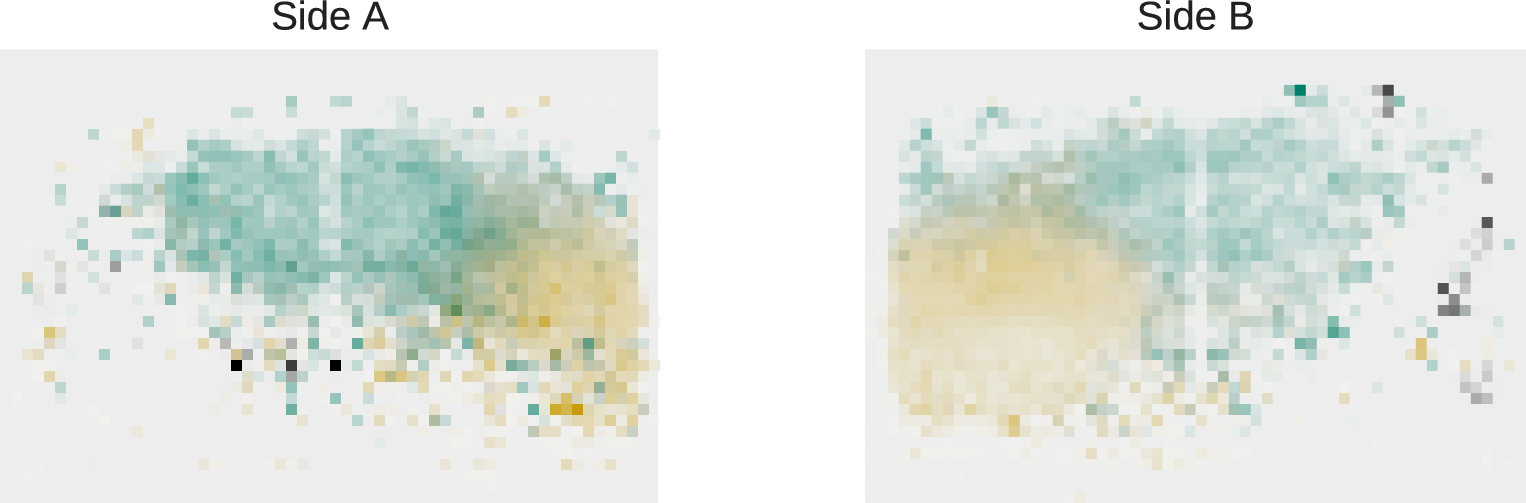
\includegraphics[width=\textwidth]{Figures/network2}
		\caption[Network 2]{Network 2}
		\label{fig:n2}
		\vspace*{5mm}
	\end{subfigure}
	%\vspace{1cm} 
	\begin{subfigure}[b]{1.0\textwidth}
		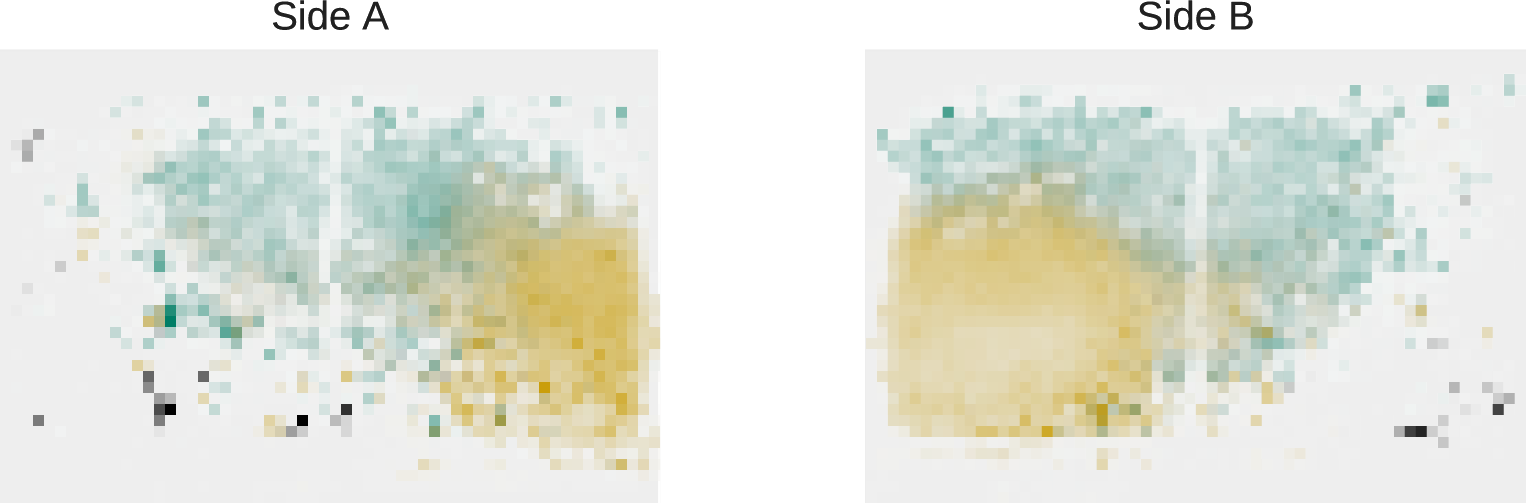
\includegraphics[width=\textwidth]{Figures/network3}
		\caption[Network 3]{Network 3}
		\label{fig:n3}
	\end{subfigure}
	\caption[Communities per network]{The \emph{green} colour represents the younger community, containing the queen, highlighted in \emph{black}. The \emph{orange} color represents the older community. The hive exit on side A is on the bottom right and on side B on the botom left.}
	\label{fig:communitiesPerNetwork}
\end{figure}


\section{Community members over time}
 The match value between the two communities in succesive time steps are calculated with formular~\ref{eq:match} and presented in figure~\ref{fig:members}. The number of bees changing from community A to community B is higher than the other way around. Which makes sense because bees change their duties while they age. this is a good indicator, but needs further investigation to be quantified.

\begin{figure}[htb]
	\centering
	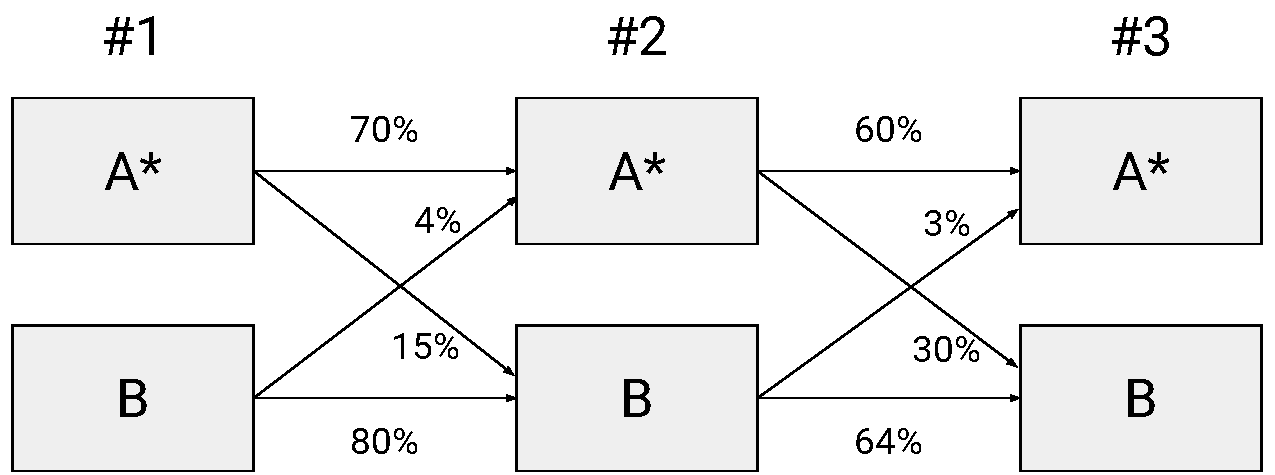
\includegraphics[width=.8\textwidth]{Figures/members}
	\caption[Community matching]{Community matching: The numbers indicate the match values. The community marked with * contains the queen and is the younger community.}
	\label{fig:members}
\end{figure}


\section{Summary}
TODO




\begin{figure}[htb]
	\centering
	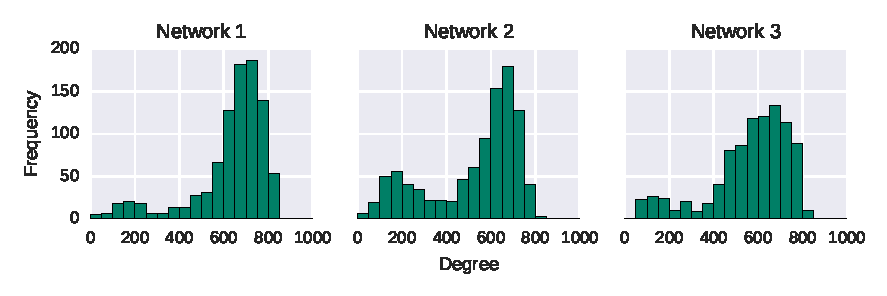
\includegraphics[width=1.0\textwidth]{Figures/stat-degreeDist}
	\caption[Degree Distribution]{Degree Distribution}
	\label{fig:statDegreeDist}
\end{figure}


\begin{figure}[htb]
	\centering
	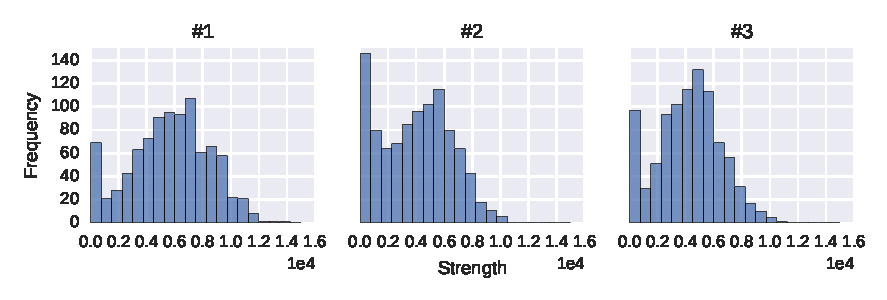
\includegraphics[width=1.0\textwidth]{Figures/stat-strengthDist}
	\caption[Strength Distribution]{Strength Distribution: Weighted Degree Distribution}
	\label{fig:statStrengthDist}
\end{figure}

\begin{figure}[htb]
	\centering
	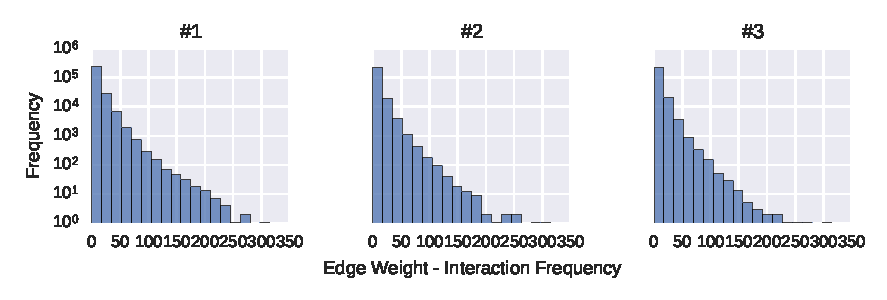
\includegraphics[width=1.0\textwidth]{Figures/stat-edgeWeightDist}
	\caption[Edge Weight Distribution]{Edge Weight Distribution - Edge weight is the contact frequency}
	\label{fig:statEdgeWeightDist}
\end{figure}


\begin{figure}[htb]
	\centering
	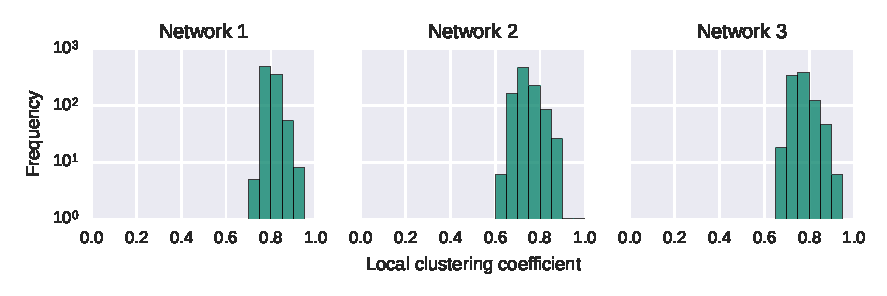
\includegraphics[width=1.0\textwidth]{Figures/stat-lccDist}
	\caption[Local clustering coefficien]{Local clustering coefficien - unweighted}
	\label{fig:lccDist}
\end{figure}


\begin{figure}[htb]
	\centering
	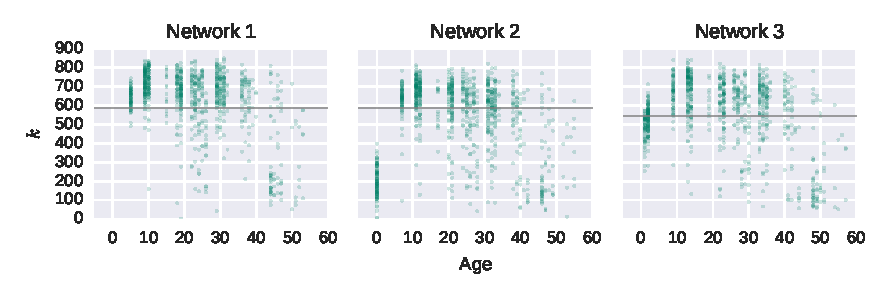
\includegraphics[width=1.0\textwidth]{Figures/stat-degreeAge}
	\caption[Degree VS Age]{Degree versus Age}
	\label{fig:degreeAge}
\end{figure}


\begin{figure}[htb]
	\centering
	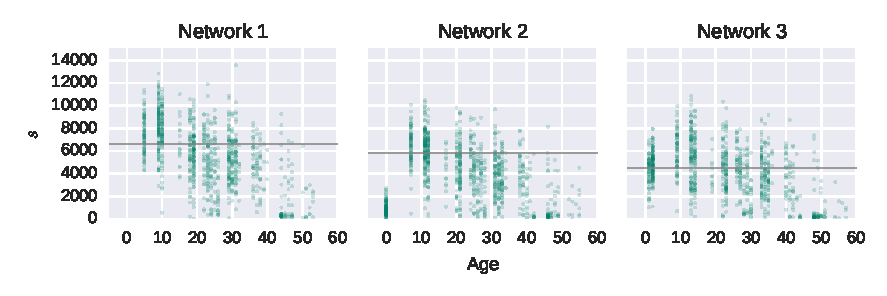
\includegraphics[width=1.0\textwidth]{Figures/stat-strengthAge}
	\caption[Strength Age]{Strength Age}
	\label{fig:strengthAge}
\end{figure}	


\begin{figure}[htb]
	\centering
	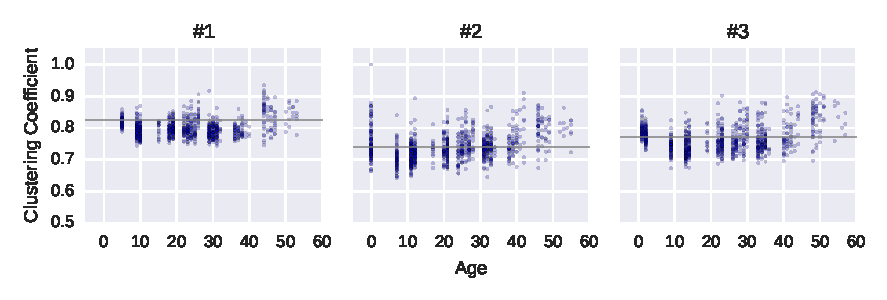
\includegraphics[width=1.0\textwidth]{Figures/stat-ccAge}
	\caption[Local clustering coefficient]{Local clustering coefficient}
	\label{fig:ccAge}
\end{figure}

%%%%%%%%%%%%%%%%%%%%%%%%%%%%%%%%%%%%%%%%%%%%%%%%%%%%%%%%%%%%%%%%%%%%%%%%%%%%%%%
%%%%%%%%%%%%%%%%%%%%%%%%%%%%%%%%%%%%%%%%%%%%%%%%%%%%%%%%%%%%%%%%%%%%%%%%%%%%%%%
%%%%%%%%%%%%%%%%%%%%%%%%%%%%%%%%%%%%%%%%%%%%%%%%%%%%%%%%%%%%%%%%%%%%%%%%%%%%%%%
%%%%%%%%%%%%%%%%%%%%%%%%%%%%%%%%%%%%%%%%%%%%%%%%%%%%%%%%%%%%%%%%%%%%%%%%%%%%%%%
\chapter{Conclusion}
\label{ch:conclusion}
%%%%%%%%%%%%%%%%%%%%%%%%%%%%%%%%%%%%%%%%%%%%%%%%%%%%%%%%%%%%%%%%%%%%%%%%%%%%%%%
%%%%%%%%%%%%%%%%%%%%%%%%%%%%%%%%%%%%%%%%%%%%%%%%%%%%%%%%%%%%%%%%%%%%%%%%%%%%%%%
%%%%%%%%%%%%%%%%%%%%%%%%%%%%%%%%%%%%%%%%%%%%%%%%%%%%%%%%%%%%%%%%%%%%%%%%%%%%%%%
%%%%%%%%%%%%%%%%%%%%%%%%%%%%%%%%%%%%%%%%%%%%%%%%%%%%%%%%%%%%%%%%%%%%%%%%%%%%%%%

The purpose of this thesis was to implement a pipeline for the extraction of time-aggregated networks using the provided high-resolution honey bee tracking data.
Moreover, the resulting weighted undirected spatial proximity networks of three consecutive time steps were analyzed regarding their network topology, community structures and the development of community members, to investigate the characteristics of honey bee colonies.

As opposed to most real world networks, these honey bee interaction networks are not scale-free networks and are characterized by a non-hierarchical topology and decentralized structure.
The small world characteristic of those networks allows for efficient communication within the bee colony.
The frequency a bee is observed inside the hive drops with increasing age.
That directly relates to the bees position in the colony network.
The detected communities relate to age-based functional groups with a spatial fidelity towards different regions of the comb. Those regions relate to the distinct type of cells and therefore to distinct tasks bees allocate.
Individual bees dynamically change functional groups as they age.

The non-hierarchical global network structure of the honey bee colony is stable over time, but its local structure is highly dynamic as individual bees change communities as they age. Those findings are aligned with previous research results and directly relate to the absence of a central authority and the decentralized organization of honey bee colonies shaped by temporal polyethism.

These network analysis results verify the definition of interaction networks by the initially chosen set of parameters and the functionality of the network pipeline in general.
The network pipeline is suitable, and it provides an excellent foundation for further investigations.

\section{Limitations}
regarding my methods, concerning implementation\\
dataset: quality, kind of a bit complex preprocessing (syncing cameras, removing invalid data, confidence), but still dead bess and almost dead bees in network\\
definition of interaction - minimum contact duration maybe was not the best idea\\
type of network spatial proximity (only proxy for interaction, no real interaction) -> maybe better contact (angle of bees similar to Mersch)/food-exchange network (interaction events), too much noise in the data\\


age distribution has some gaps (tagging not on weekends)-> not sure about it effects\\
context, missing domain knowledge, working in an interdisziplinary teams\\

\section{Future Work}
(1) recommendations for further studies, (2) recommendation for change\\
each recommendation should directly trace a direct conclusion\\

investigate: correlation of density and time, upper bound? or 100\% density after some X frames?\\
are communities robust regarding pipeline parameters maximum distance, minimum contact duration, window size (yes they are, tested for some values, but not systhematically)\\
pipelie parameters (maximum distance, minimum contact duration, window size) effects on network properties (degree, strength,lcc, edgeweights) ... tested but not systematically only some values and only window size up to one hour, should be done more systematically\\
compare the networks to random geometric graph~\cite{rgg2002} and model a walking bee as a random walker\\
so far nodes are attributed with only age and detection frequency, add other stuff, e.g. average speed, total distance traveled\\
compute centrality measures per community\\
weighted edges, should also inpect weighted versions of node measures (this was a bit to complicated, already implemented weighted version in networkX and igraoh do favour weights over number of hops, should look at~\textcite{opsahl2010node}, but depending on what you want to investigate you have to choose the $\alpha$)\\
compare analysis results to NON artifical bees networks\\
investigate different granularities (size of time window)\\
study longer time period not only 5 days\\
normalized edge weight (SRI - Simple Ratio Index, SRI measures
the proportion of times two individuals were seen
together out of the total number of times those individ-
uals were observed, by \textcite{croft2008exploring}) or normalized degree and stuff by frequency of detection\\
apply network reduction algorithm to reduce density and noise, by applying (no simple edge thresholding), disparity filter~\textcite{serrano2009extracting}

\vspace{2cm}
more data does not mean better analysis, one have to ask good questions, develop specialized hypothesis, a lot of options\\
explorative analysis approach difficult with data from animals I do not know, maybe easier with 'human' data (missing domain data)\\
alienation: automatic tracking -> no relation to the data or how the data was collected or animals\\
just applying network method to new research fields, sometimes just replicates known facts, Ending with: Zitat Krause (Buch)
%---------------------------------------------------
%----- Bibliography
%---------------------------------------------------
\printbibliography

%---------------------------------------------------
%----- Directories   
%---------------------------------------------------

\addcontentsline{toc}{chapter}{\listfigurename}
\listoffigures
\clearpage %\cleardoublepage %for openright
\addcontentsline{toc}{chapter}{\listtablename}
\listoftables
\clearpage %\cleardoublepage %for openright
%\lstlistoflistings

%---------------------------------------------------
%----- Appendix   
%---------------------------------------------------
\appendix
\chapter{Appendix Stuff}
\label{ch:appendix}

\begin{table}
\centering
\caption[XXX]{\textbf{XXX} \url{https://docs.google.com/spreadsheets/d/1eKuPU-XmqwrHkS_5-TgS8UnO5O-Hwe1kyRIpareywP4/edit?usp=sharing}}
\label{tab:studies}
\vspace*{5mm}
\begin{tabular}{ccc}
	\toprule
	{}  & TODO & TODO \\
	\midrule

	x & x & x\\
	x & x & x\\
	\bottomrule
\end{tabular}
\end{table}

[TODO: Table with studies related to social insects and bees and manual and automatic tracking.]

[TODO: Figure: Maintance and Faliour Days, also maybe timeline for each camera]

[TODO: ]
\backmatter

\end{document}